\section{Overview of neutron \tot\ experiments}

Neutron scattering is a direct, Coulomb-insensitive tool for probing the nuclear
environment. The simplest measurement of neutron interaction with a nucleus,
the neutron total cross section \tot, provides fundamental information about
nuclear size and the ratio of elastic-to-inelastic components of nucleon 
scattering. Additionally, \tot\ data are connected to a variety of nuclear
properties of great interest including the neutron skin of neutron-rich nuclei
\cite{Mahzoon2017} and thus the density dependence of the symmetry energy $L$,
essential for an accurate neutron star equation-of-state (EOS)
\cite{Fattoyev2012, Vinas2014, Brown2000}.

By scattering secondary radioactive beams off of hydrogen targets in \gls{inverse
kinematics}, proton-scattering experiments are possible even on highly unstable
nuclides. In contrast, because neutrons themselves must be generated as a
secondary radioactive beam, neutron-scattering experiments are restricted to
normal kinematics and \tot\ measurements are possible only for relatively stable
nuclides that can be formed into a target. At present, \tot\ measurements above
the resonance region on nuclides with short half-lives (shorter than the timescale of
days) are technically infeasible for this reason, though a handful have been carried out on
samples with half-lives in the tens to thousands of years \cite{Poenitz1983,
Phillips1980, Foster1971}.

Traditionally, \tot\ measurements have relied on analog electronics for processing and
recording events, techniques that suffer from a large per-event deadtime of
up to several $\upmu$s. For a state-of-the-art intermediate-energy \tot\ measurement
with dozens or hundreds of energy bins, achieving statistical uncertainty at the
level of 1\% requires a thick sample to attenuate a sizable fraction of the
incident neutron flux.
For cross sections in the 1-10 barn range, this means
sample masses of tens of grams \cite{Finlay1993, Abfalterer2001}.
Producing an isotopically-enriched sample of this size is often
prohibitively expensive. This explains the lack of data for isotopically-resolved
\tot\ measurements from 1-300 MeV even for
closed-shell isotopes of special importance like $^{3,4}$He, $^{64}$Ni, and
$^{204}$Pb (see Table \ref{IsotopicCrossSectionTable}).

\begin{table}[ht]
    \caption[Selected results from a literature study of isotopically-
        resolved \tot\ data using the EXFOR database \cite{EXFORDatabase}]
        {Selected results from a literature study of isotopically-
        resolved \tot\ data using the EXFOR database \cite{EXFORDatabase}
        For the heaviest and lightest stable nuclides in each closed shell in Z, all
        datasets falling at least partially within 1-500 MeV are shown. For elements
        whose natural abundance is $>$90\% of a single isotope (e.g.,
        96.9\% of $^{\text{nat}}$Ca is $^{40}$Ca), \tot\ data on the natural
        target was included as ``isotopic".}
    \label{IsotopicCrossSectionTable}
    \begin{center}
        \begin{tabular}{ c c c c }
            \hline
            Isotope & Nat. Abund. & Energy Range & Reference \\ & [\%] & [MeV] & \\

            \hline

            $^{3}$He & $2\times 10^{-4}\%$ & $1.5 - 40$ & \cite{Haesner1983}\\
            $^{4}$He & $>99.9\%$ & $0.7-30$ & \cite{Goulding1973}\\
            & & $2-40$ & \cite{Haesner1983}\\
            & & $77-151$ & \cite{Measday1966}\\

            $^{16}$O & $99.8\%$ & $0.2-49$ & \cite{Perey1972}\\
            & & $5-600$ & \cite{Finlay1993}\\

            $^{18}$O & $0.20\%$ & $0.1-2.5$ & \cite{Vaughn1965}\\
            & & $2.5-19$ & \cite{Salisbury1965}\\

            $^{40}$Ca & $96.9\%$ & $<0.1-6.4$ & \cite{Johnson1973}\\
            & & $5.3-560$ & \cite{Abfalterer2001}\\

            $^{48}$Ca & $0.187\%$ & $0.6-5.2$ & \cite{Harvey1985}\\
            & & $12-276$ & \cite{Shane2010}\\

            $^{58}$Ni & $68.1\%$ & $<0.1-68$ & \cite{Perey1993}\\

            $^{64}$Ni & $0.926\%$ & $14.1$ & \cite{Dukarevich1967}\\

            $^{112}$Sn & $0.97\%$ & $<0.1-1.4$ & \cite{Timokhov1989}\\
            & & $14.1$ & \cite{Dukarevich1967}\\

            $^{124}$Sn & $5.79\%$ & $0.3-5.0$ & \cite{Harper1982}\\
            & & $5.1-26$ & \cite{Rapaport1980}\\

            $^{204}$Pb & $1.4\%$ & $<0.1-27$ & \cite{Carlton2003}\\

            $^{208}$Pb & $52.4\%$ & $<0.1 - 695$ & \cite{Harvey1999}\\
            & & $5-600$ & \cite{Finlay1993}\\

            \hline
        \end{tabular}
    \end{center}
\end{table}

In the 1990s, a comprehensive series of measurements were made at the Weapons Neutron Research (WNR)
facility of the Los Alamos Neutron Science Center (LANSCE) on a wide battery of samples from Li to
Pb \cite{Finlay1993, Abfalterer2001}, some isotopically-separated. Twenty years
later, the measurements on \caAughtEight \cite{Shane2010} were the first 
to employ newly-available digital-signal-processing technology to reduce the deadtime associated
with processing each event and thus reduce the needed sample size. In 2015, we
embarked on a systematic campaign to measure neutron \tot\ across the widest possible energy range
for the heaviest and lightest stable isotopes in the Z = 8, Z = 28, and Z = 50 closed shells.

\section{Detector Construction}
Because neutrons carry no charge, they penetrate materials much further than protons and do not
deposit energy continuously along their path. Further, when neutrons do interact with nuclei in
detector materials, the energy transferred does not correspond linearly to the neutron energy. Thus
assigning the correct energy to a scattered neutron is far from trivial. The main approach to
energy determination for fast neutrons is by time-of-flight, as evidenced by state-of-the-art
neutron detector arrays including MoNA \cite{MoNA}, VANDLE \cite{VANDLE}, and
NeuLAND\cite{NeuLAND}.

\begin{figure}[ht]
    \centering
    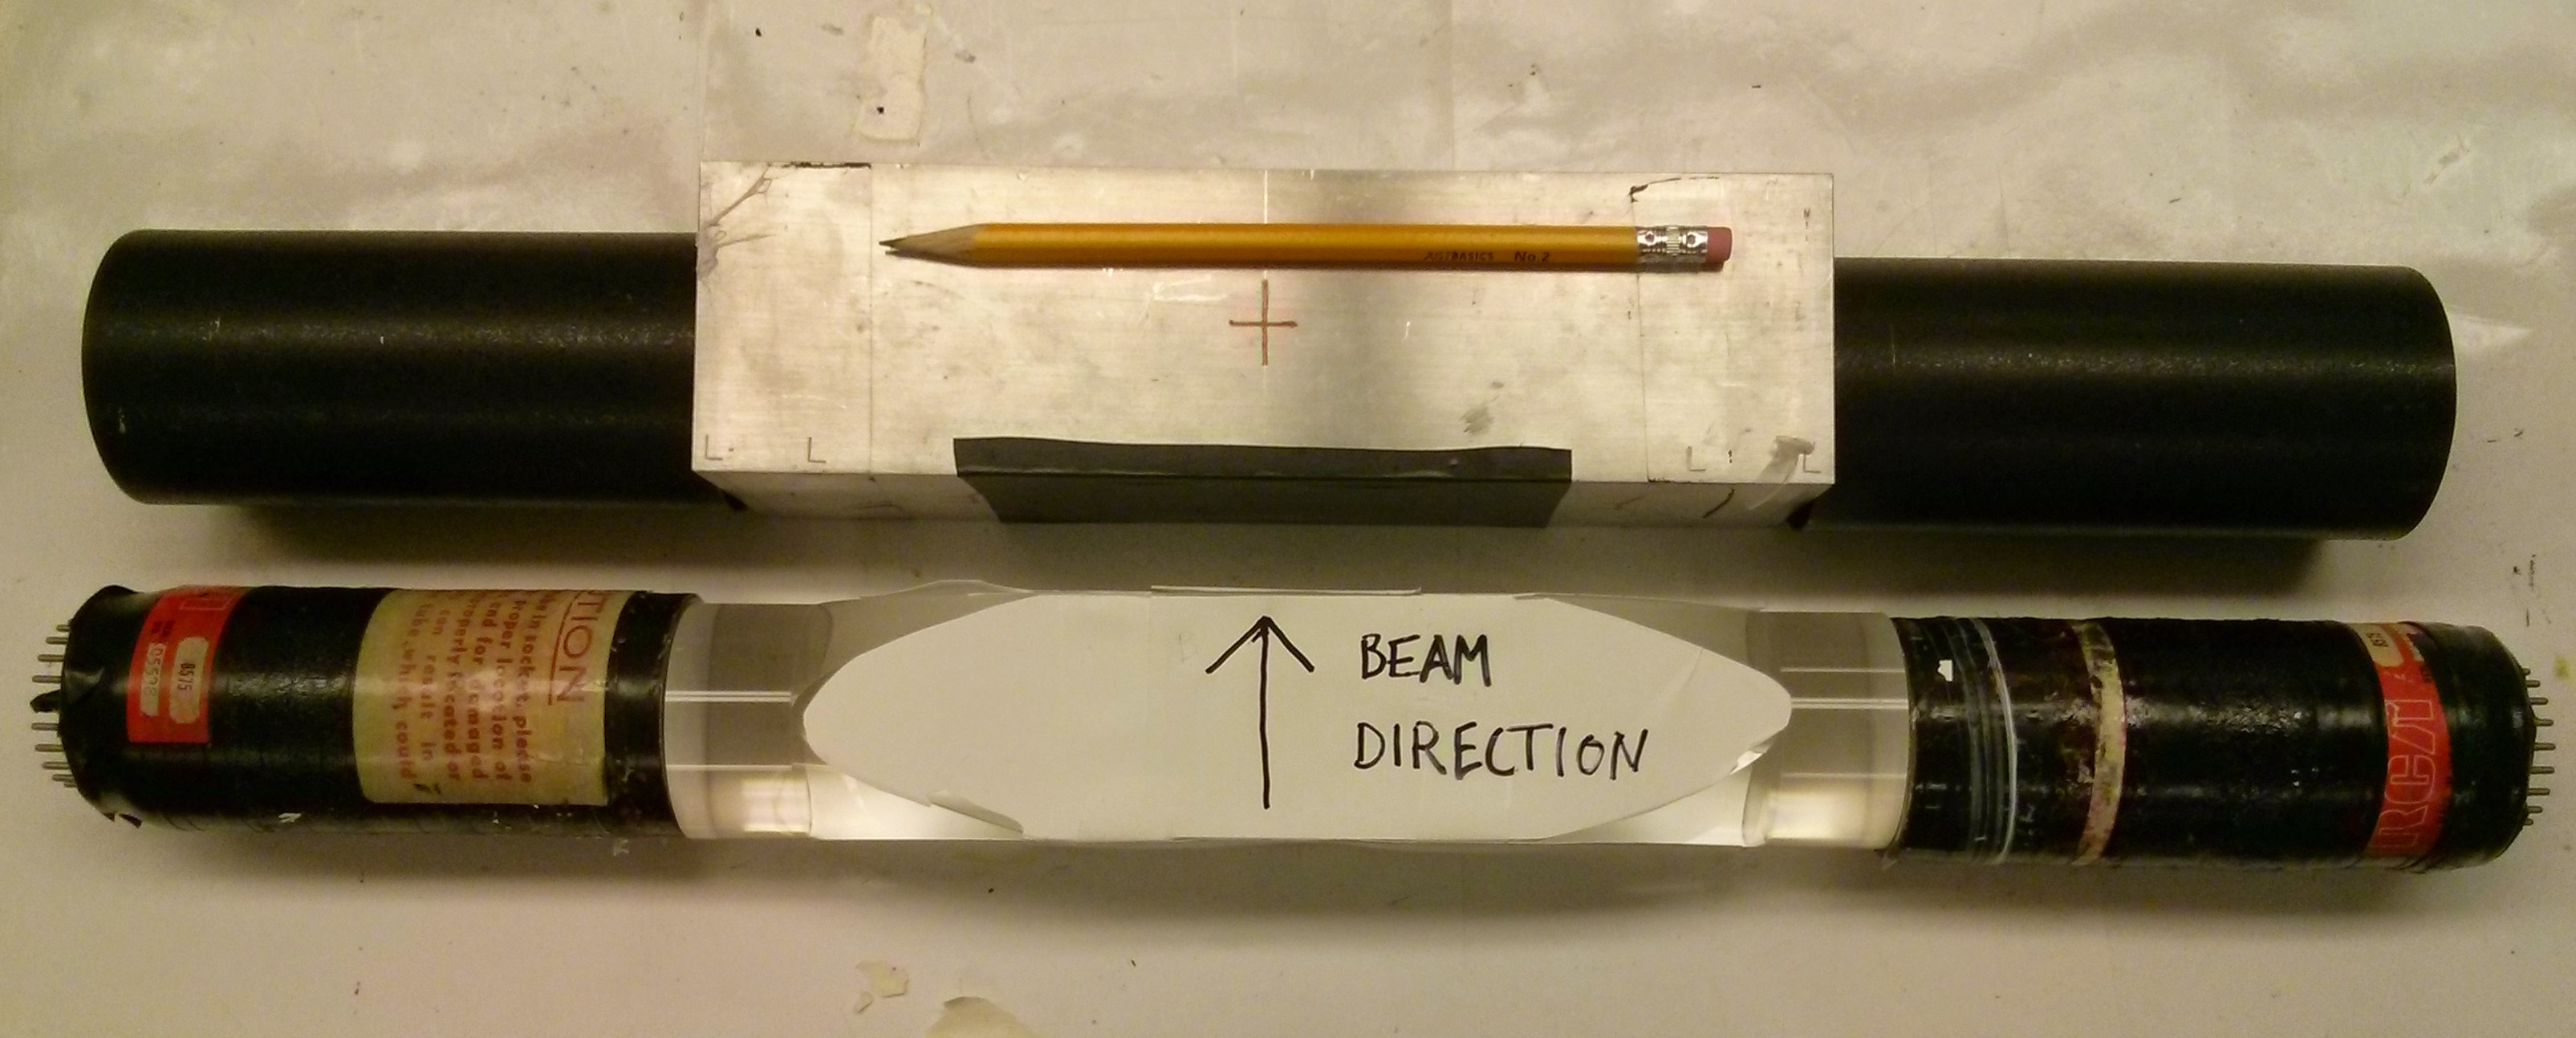
\includegraphics[width=0.8\textwidth]{figures/Scintillator_disassembled.jpg}
    \caption[Time-of-flight detector partially assembled]
    {One of three time-of-flight detectors, partially assembled, with pencil for scale.
        The aluminum casing and Delrin phototube sleeves are at top, and the
        scintillator (beneath the beam direction arrow), lightguides, and phototubes, at
        bottom. The detector described in the text has a thinner scintillating plastic
    element (1 inch thick) and tapered lightguides to match.}
    \label{TOFDetectorDisassembled}

    \vspace*{\floatsep}

    \centering
    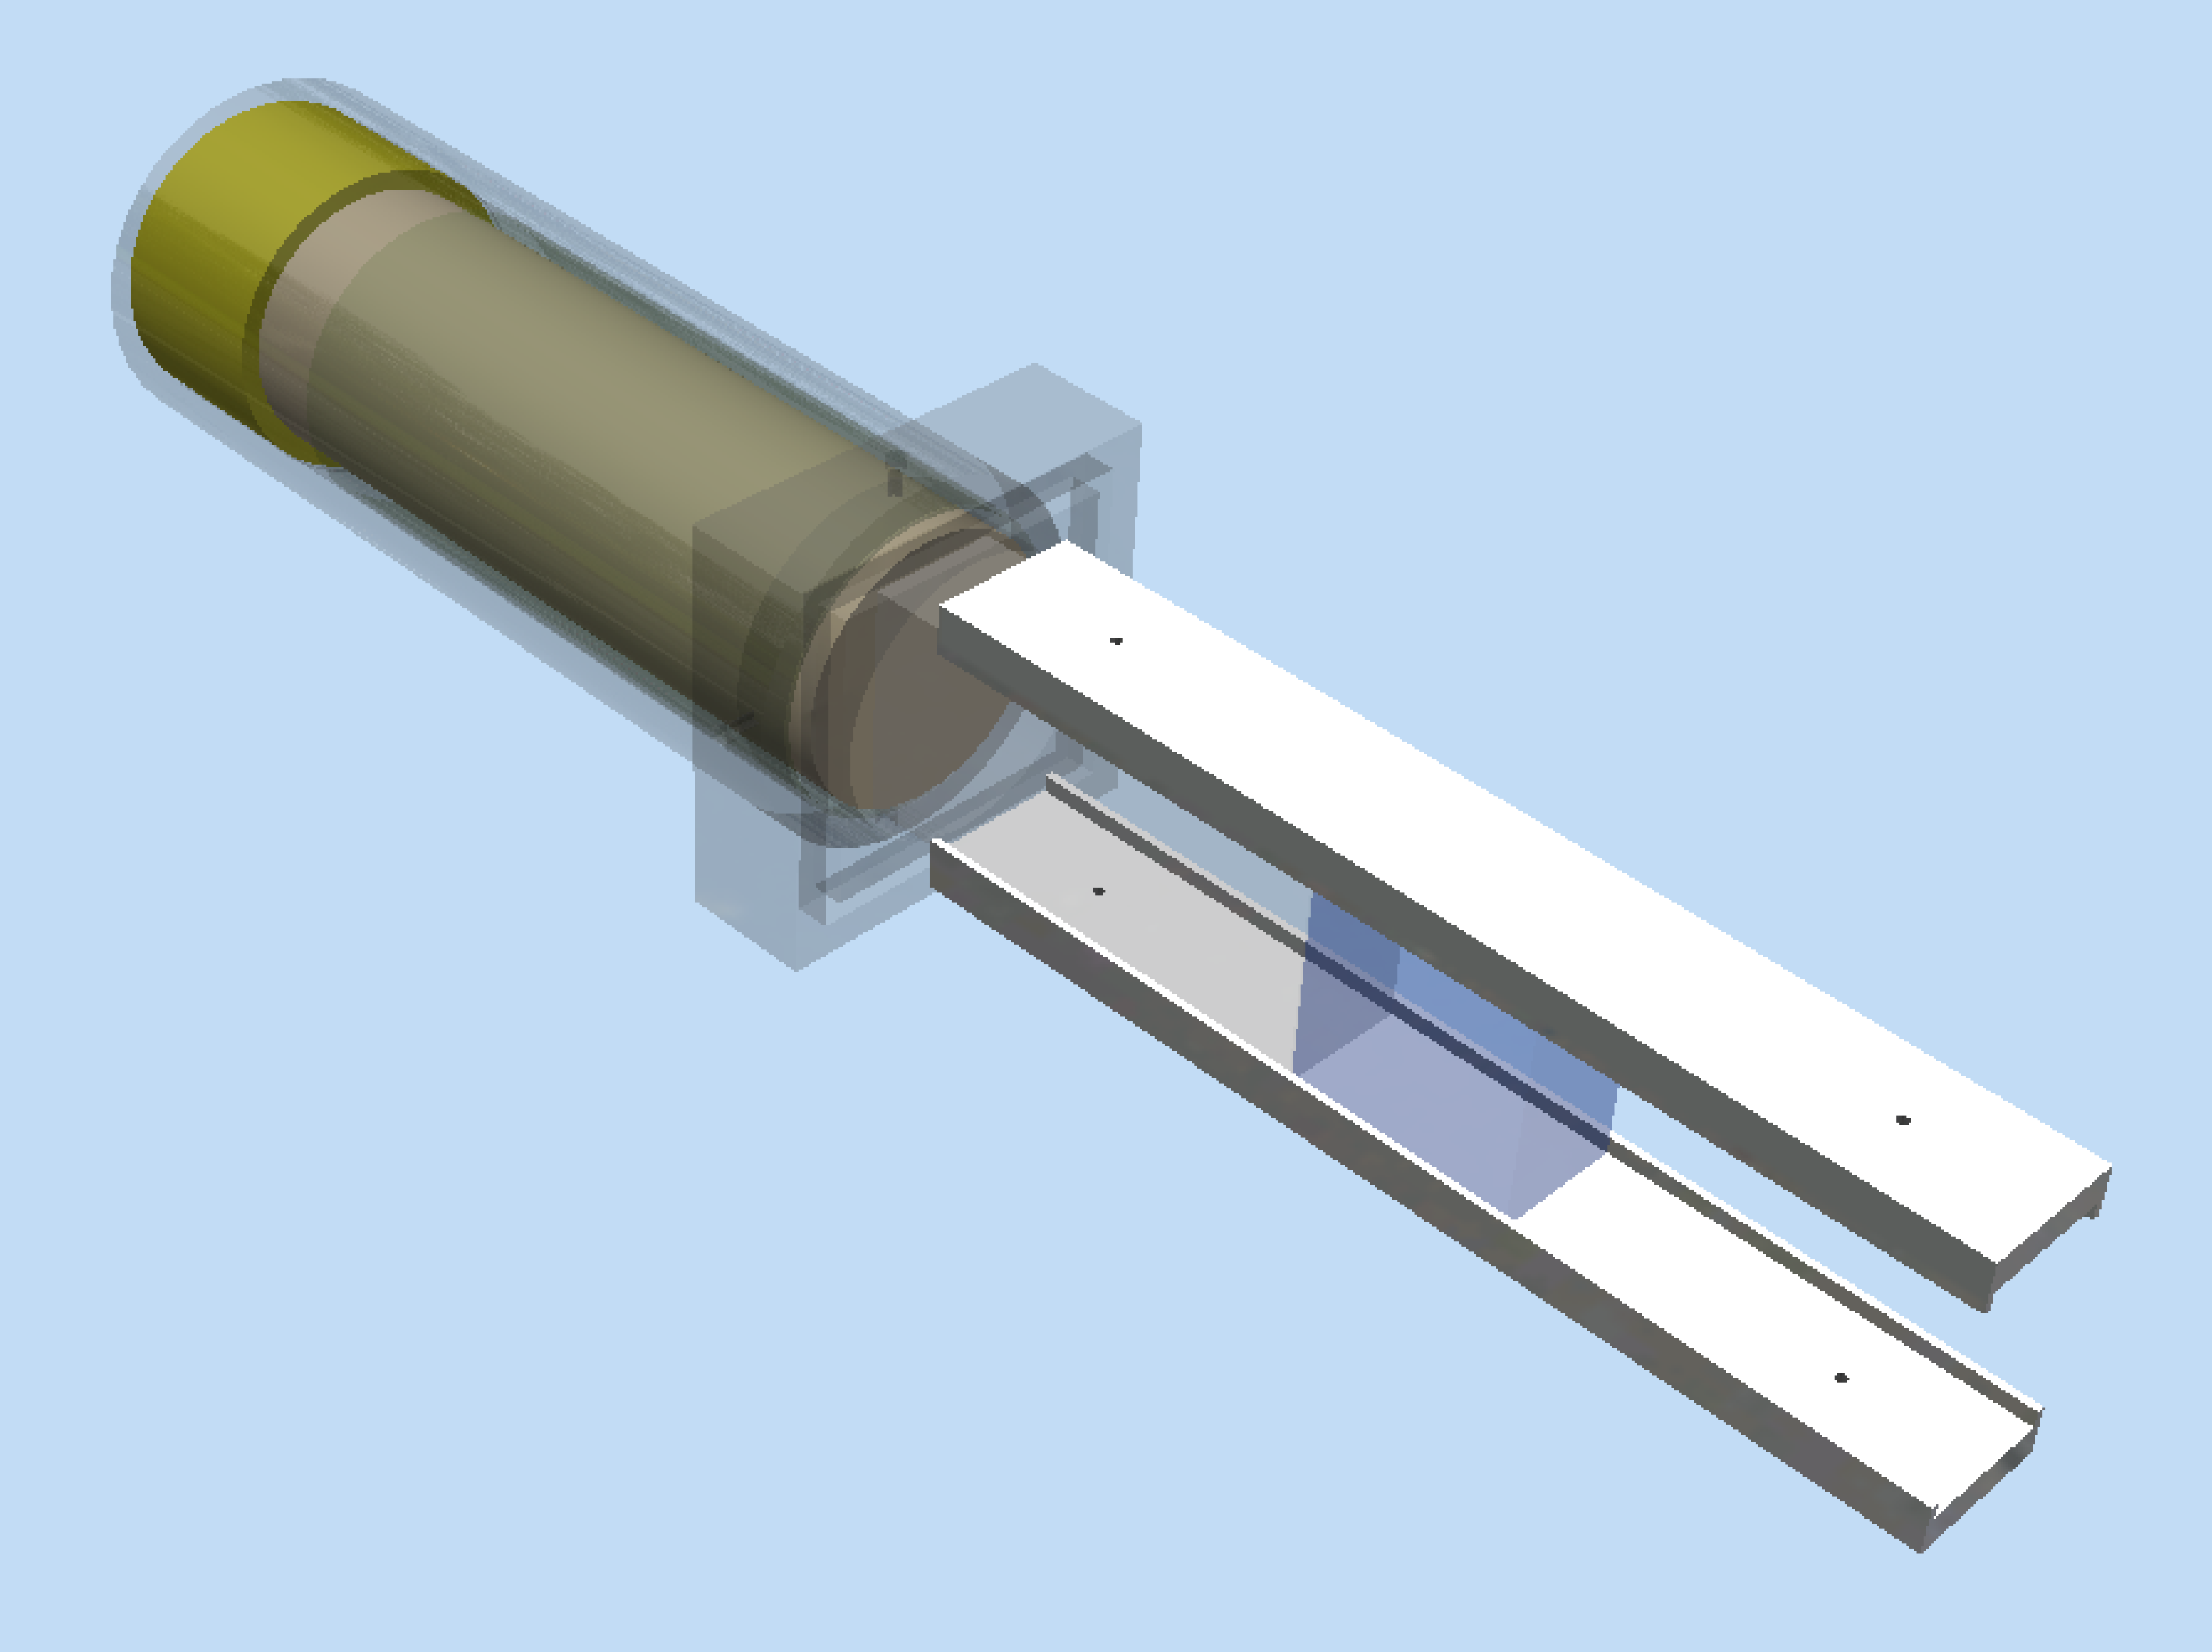
\includegraphics[width=0.8\textwidth]{figures/TimeOfFlightCAD.png}
    \caption[Cutaway CAD figure of time-of-flight detector.]
    {
        Cutaway CAD figure of time-of-flight detector described in the text. The 
        1-inch-thick scintillating plastic element is visible in the middle of the aluminum 
        housing brackets, and the light-tight sleeve for the phototube is visible on
        the left.
    }
    \label{TOFCAD}
\end{figure}

Figure \ref{TOFDetectorDisassembled} shows a time-of-flight detector used in one
of our neutron \tot\ measurements. A 2 inch x 2 inch x 1 inch block of BC-400 fast
plastic scintillator is coupled to two transparent
BC-800 adiabatic lightguides with RTV rubberized adhesive. These components were encased
in an aluminum structural housing. On the distal end of the lightguides, Hamamatsu 1668
photomultiplier tubes were connected with optical grease and enclosed by
$\upmu$-metal shielding, used to prevent external magnetic fields from affecting photoelectrons.
Phototube signals and high voltage were supplied by a phototube base attached to the back of each
phototube. To hold the phototubes, fitted black Delrin sleeves (shown on the
left side of the CAD cutaway Fig. \ref{TOFCAD}) were custom-made to apply slight
compression, keeping the optical surfaces in good contact. The entire assembly
is 24 9/16'' in length.

\section{Sample Preparation}
Where possible, the \tot\ samples were formed as right
cylinders 8.25 mm in diameter and ranging from 10-27 mm in length (see
Table \ref{SampleCharacteristics} for sample characteristics and Fig. \ref{SamplesImage}
for sample images). A natural-abundance sample
was also prepared for each element for use in benchmarking to already-existing
literature neutron \tot\ values. During the experiment, the samples were inserted
into styrofoam sleeves and seated in the cradles of the sample
changer, described below. This design minimizes the amount of non-target mass proximate to the
neutron beam path that could cause unwanted neutron scattering. For all O, Ni,
and Sn samples, the areal densities of atoms in the sample, the relevant quantity for cross section
measurements, differ by less than 1\%.

For the oxygen isotopes, isotopically-enriched water samples were prepared to
increase the areal density of O in the sample volume and for ease of handling.
After measurement, the
extremely-well-known H neutron \tot\ could be subtracted to yield the O \tot\ values.
This technique is also used by \cite{Vaughn1965, Salisbury1965}; cf.  with
results using ZnO and BeO of \cite{Finlay1993}.
Because the natural abundance of \oSix\ in H$_{2}$O is $>$99\%, a sample of
ordinary distilled water was used for the H$_{2}$\oSix\ sample. For H$_{2}$\oEight,
we used distilled water enriched to $>$99\% in \oEight\ from
[manufacturer]. Both samples were enclosed in brass vessels with thin
(0.002") brass endcaps, to minimize neutron attenuation. At the temperature and
altitude of the experimental facility, the amount of dissolved gas and ions
in the water samples were small enough to have no effect on the measurement.

The isotopic Sn samples were prepared by melting highly-enriched foils to
800 C in a tube furnace, cooling to ambient temperature, and pressing the ingots
to the desired cylindrical shape in a tempered die. To reduce formation of tin
oxide during melting, the samples were melted in vitreous carbon crucibles
and kept under a reducing atmosphere (90\% Argon/ 10\%H2) while at elevated
temperatures. Of the 4.9 grams of \snTwelve\ used to prepare the sample,
3.5 grams were from a semi-permanent loan from the group of Lee Bernstein from LLNL
and the remainder we purchased from Isoflex Corp. All of the 5.8 grams of \snFour\
were purchased from Isoflex. The \snNat\ sample was prepared by melting and
pressing analytical-grade Sn shot from Mallinckrodt Corp. Loss of isotopic
material during the manufacturing process was minimal.

The natural and isotopic Ni samples were prepared by [insert name] at Oak Ridge
National Lab (ORNL) to match the diameter of our Sn samples.

Due to its poor machining properties, the Rh sample was prepared by
stacking a series of thin rhodium disks instead of manufacturing a
fused cylinder. Four disks of 99.9\% pure natural (monoisotopic) Rh metal were purchased from
Goodfellow Corp. These were corralled with a
plastic sleeve with open ends, similar to the styrofoam sleeves used for the Ni
and Sn samples, to match the $\frac{3}{4}$-inch-diameter cradles of the sample changer
\ref{RhodiumSample}.
This kept the discs snugly in series and perpendicular to the beam path.

Lastly, two natural-abundance graphite samples of different lengths and one
natural-abundance Pb sample, all with the same diameter as the Sn and Ni samples, were
prepared. These samples were used to benchmark the total cross sections
measured at LANSCE by comparison with previous measurements of the C and
Pb total cross sections available in the literature
(\cite{Finlay1993,Abfalterer2001}). In addition, the low-energy neutron \tot\ resonance
structure of the C samples served a crucial role in fixing the exact distance
of the time-of-flight detector as detailed in Chapter \ref{TCSAnalysis}.
Before use, the C samples were baked in an oven for several
hours to remove adsorbed water.

\begin{table}[ht]
    \caption[Physical characteristics of samples used for neutron \tot\
    measurements]
    {
        For isotopically-enriched samples, the natural abundance
        of the enriched isotope and the isotopic fraction of the sample are
        given. To calculate cross sections, the relevant ``sample thickness" is the areal
        density of nuclei $\rho_{\text{areal}}$, equivalent to
        the (volumetric) density times the length of the sample. For liquid
        samples H$_{2}^{\text{nat}}$O, D$_{2}^{\text{nat}}$O, and H$_{2}^{18}$O,
        the length and diameter listed are for the interior of the vessels
        used to hold the samples and the masses given are calculated based on 
        literature values for the density of each sample at 25\textdegree{}C.
        Our samples are generally much smaller than those used in previous
        measurements; for comparison, the Ni and Sn samples used in \cite{Abfalterer2001,
        Finlay1993} had areal densities of 1.515 and 0.5475
        $\frac{mol}{cm^{2}}$, respectively (12.7 and 6.5 times larger than our
        Ni and Sn samples).
    }
    \label{SampleCharacteristics}
    \begin{center}
        \begin{tabular}{ c c c c c c c }
            \hline
            Isotope & Length & Diameter
            & Mass & $\rho_{\text{areal}}$ & Nat. Abund. & Sample Purity\\
                 & [mm] & [mm] & [g] & [$\frac{mol}{cm^{2}}$] & [\%] & [\%]\\
            \hline

            $^{\text{nat}}$C & 13.66(2) & 8.260(5) & 1.2363
            & 0.1921(1) & - & -\\
            $^{\text{nat}}$C & 27.29(2) & 8.260(5) & 2.4680
            & 0.3835(2) & - & -\\

            H$_{2}$$^{\text{nat}}$O & 20.00(1) & 8.92(1) & 1.2461 & 0.1107(3) & - &
            - \\
            D$_{2}$$^{\text{nat}}$O & 20.00(1) & 8.92(1) & 1.3852 & 0.1107(3) & - &
            - \\
            H$_{2}$$^{18}$O & 20.00(1) & 8.92(1) & 1.3844 & 0.1107(3) & 0.20 & 99\\

            $^{58}$Ni & 7.97(3)& 8.18(2) &
            3.6438 & 0.1197(3)& 68.1 & 99.6 \\
            $^{\text{nat}}$Ni & 8.00(3) & 8.20(2) &
            3.6898 & 0.1192(3)& - & -\\
            $^{64}$Ni & 7.96(2) & 8.20(4) &
            3.9942 & 0.1192(6) & 0.93 & 92.2\\

            $^{103}$Rh & 2.03(1) & 10.20(2) & 2.8359 & 0.02426(4) & 100 & 99.9\\

            $^{112}$Sn & 13.65(3) & 8.245(5) &
            4.9720 & 0.08332(5) & 0.97 & 99.9\\
            $^{\text{nat}}$Sn & 13.68(3) & 8.245(5) &
            5.3263 & 0.08414(5) & - & -\\
            $^{124}$Sn & 13.73(3) & 8.245(5) &
            5.5492 & 0.08399(5) & 5.79 & 99.9\\

            $^{\text{nat}}$Pb & 10.07(2) & 8.27(1) & 6.130 &
            0.05508(6) & - & -\\

            \hline
        \end{tabular}
    \end{center}
\end{table}

\begin{figure}[ht]
    \centering
    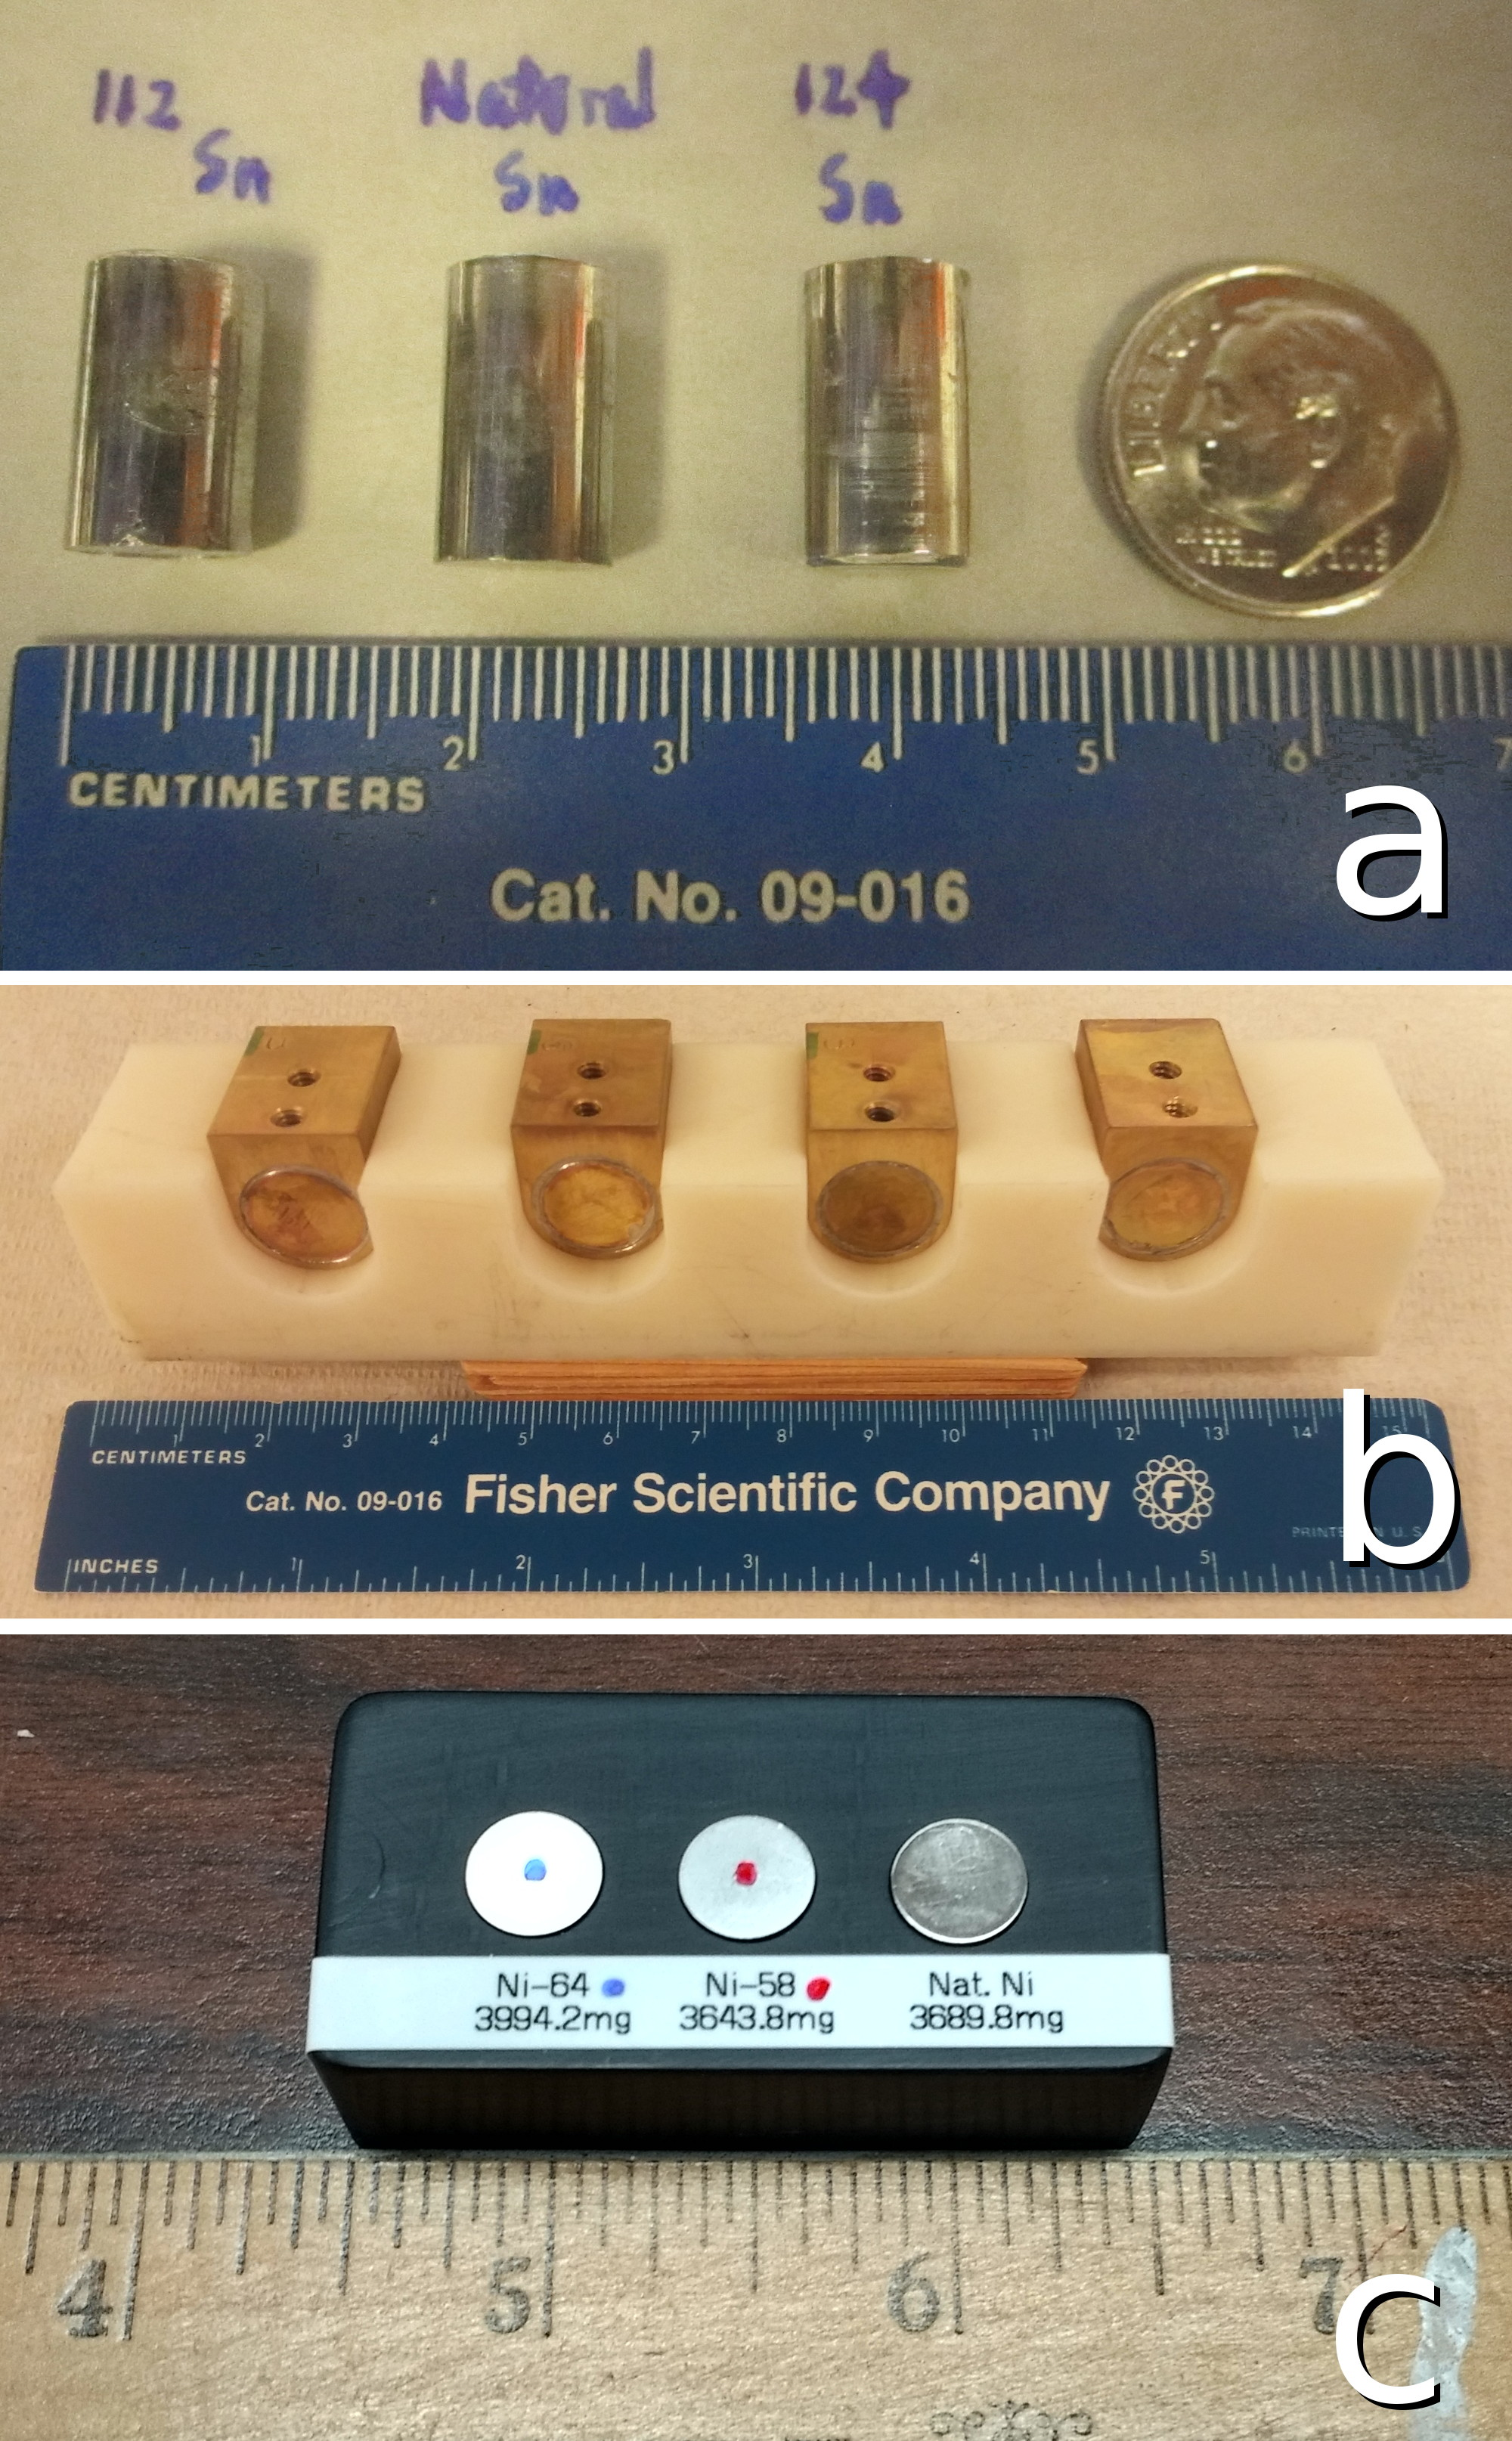
\includegraphics[width=0.5\textwidth]{figures/AllIsotopicSamples.jpg}
    \caption[${^{112,\text{nat},124}}$Sn, $^{{\text{nat}, 18}}$O, and ${^{58,\text{nat},64}}$Ni
samples used for neutron \tot\ measurements]
{
    ${^{112,\text{nat},124}}$Sn (section a), H$_2^{{\text{nat}, 18}}$O (section
    b), and ${^{58,\text{nat},64}}$Ni
    samples (section c) used for neutron \tot\ measurements, with rulers for
    scale. Brass vessels were used to hold the water samples.
}
    \label{SamplesImage}

    \vspace*{\floatsep}

    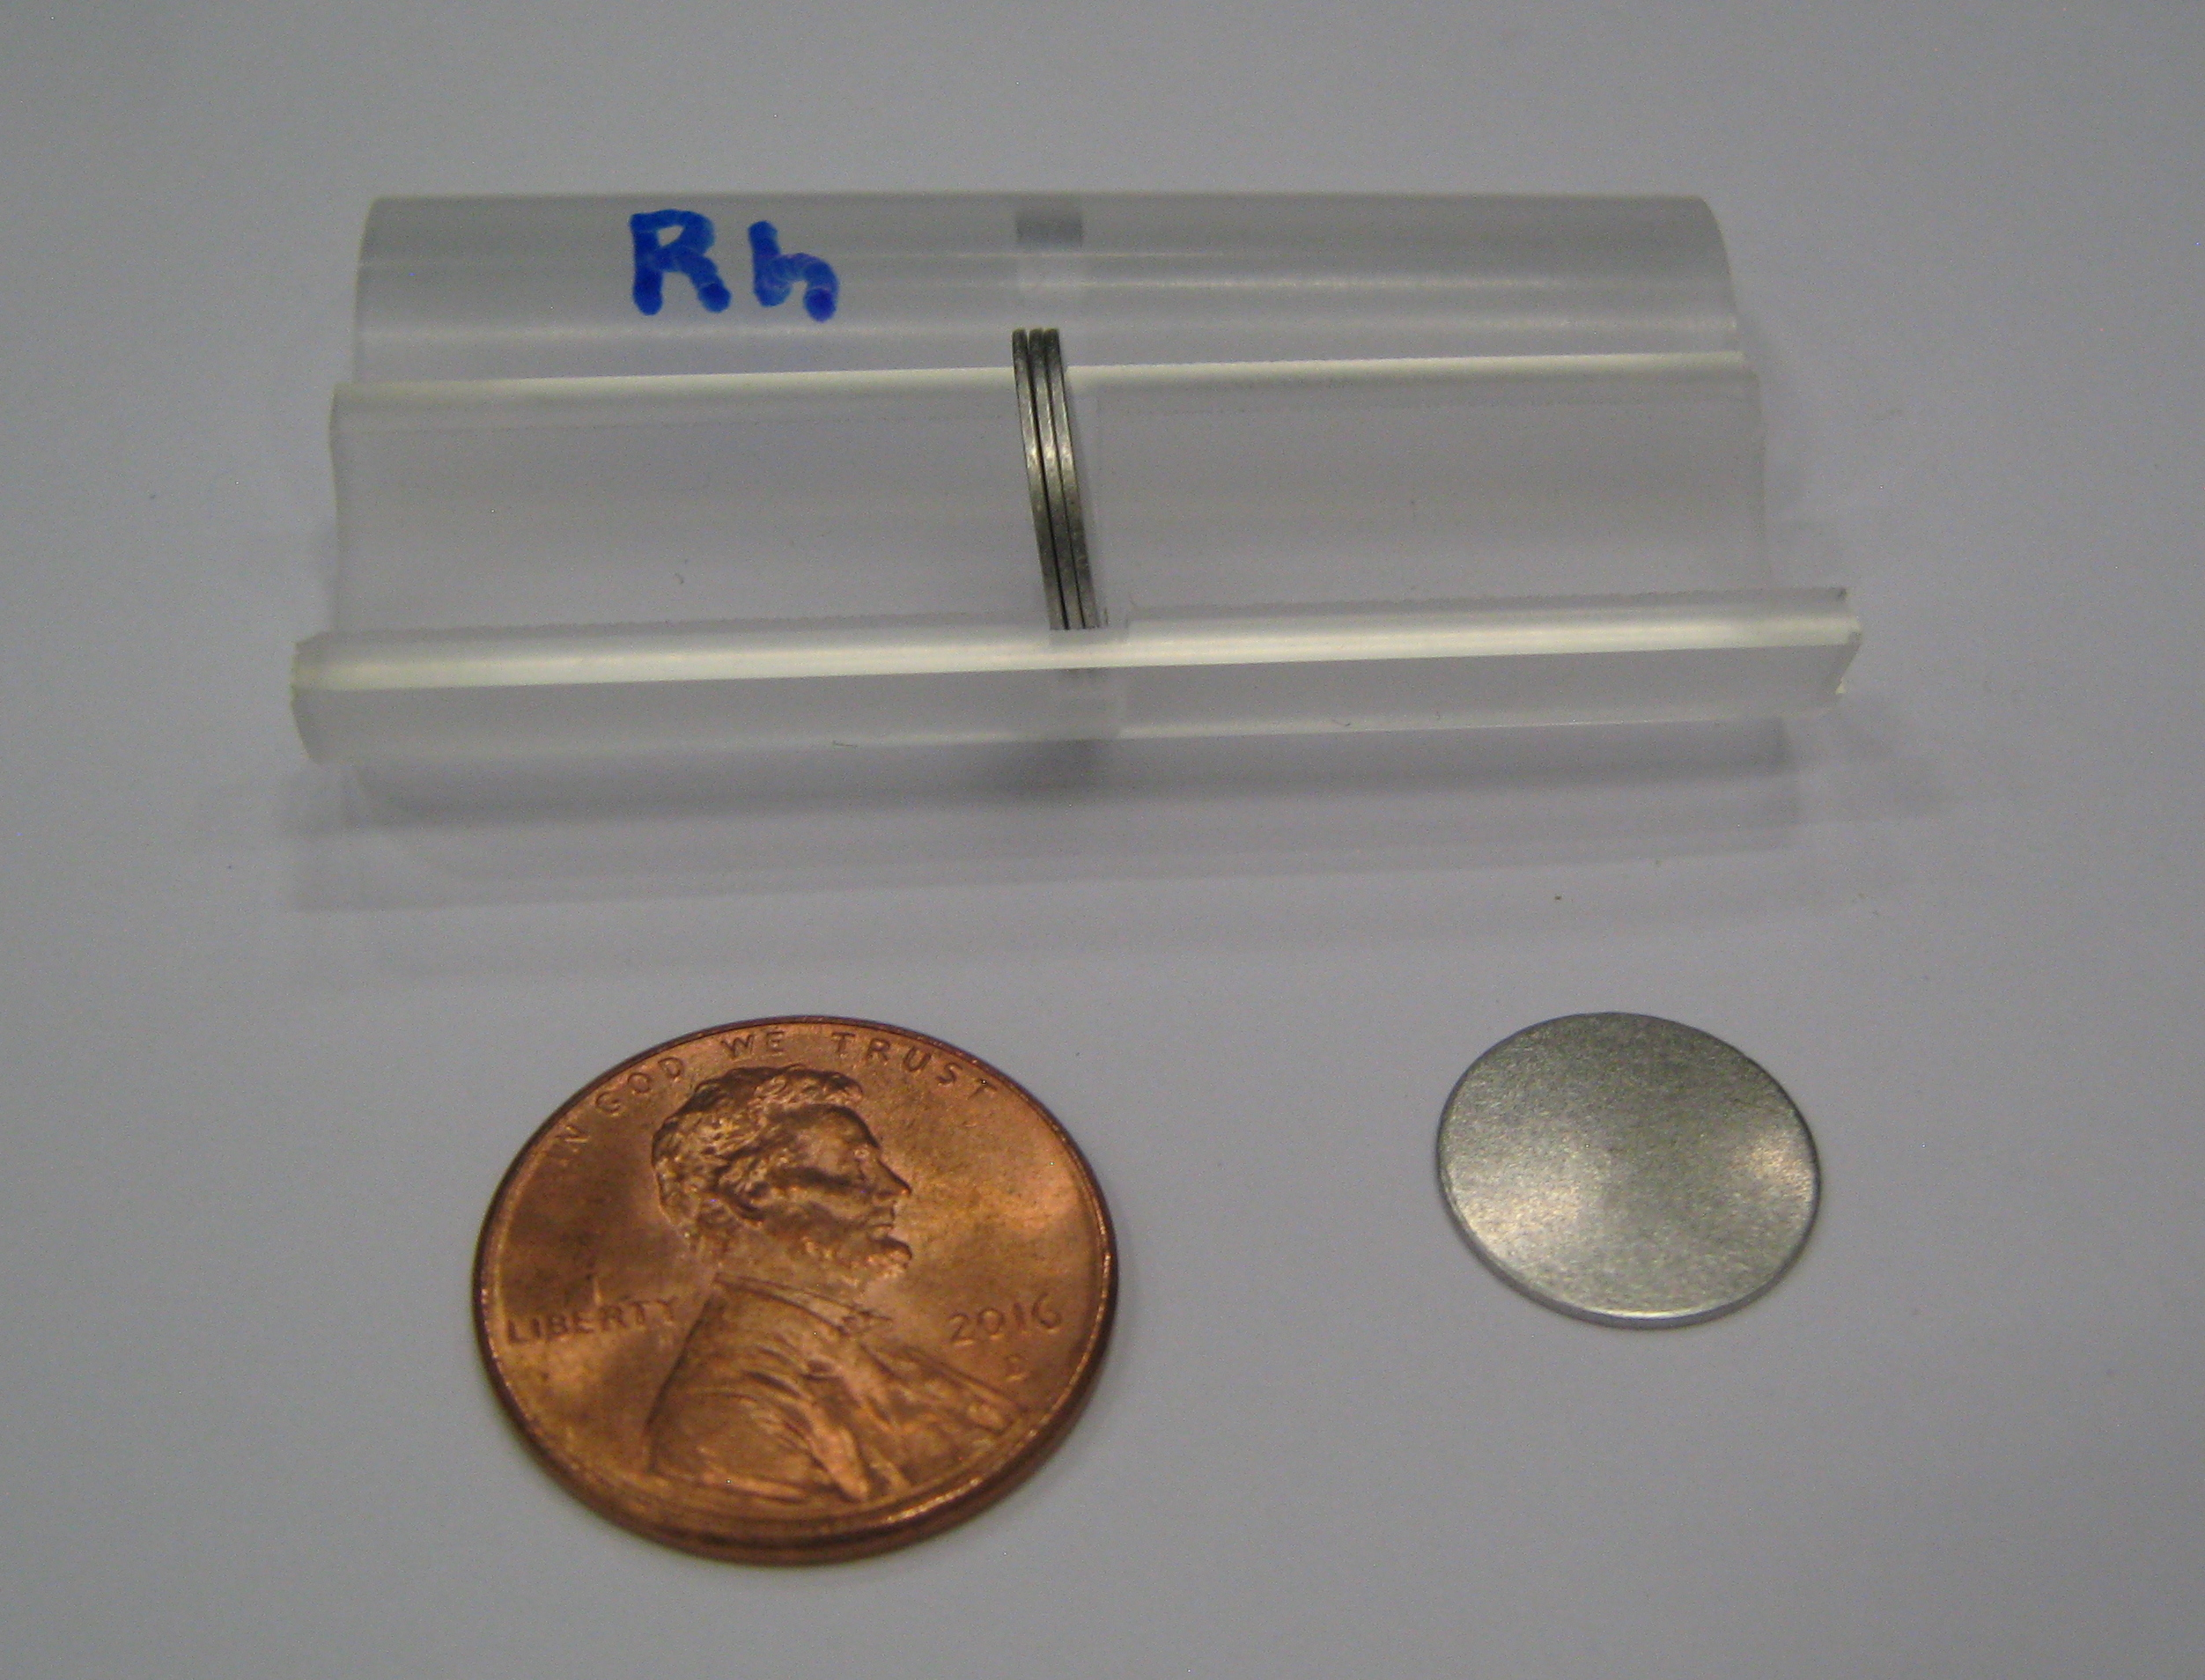
\includegraphics[width=0.5\textwidth]{figures/RhodiumSample.jpg}
    \caption{\rhThree\ sample used for the neutron \tot\ measurements}
    \label{RhodiumSample}
\end{figure}

\section{Experimental Facility at LANSCE}
All neutron \tot\ measurements were carried out at the 15R
beamline of the Weapons Neutron Research (WNR) facility at the Los Alamos
Neutron Science Center (LANSCE) over two run cycles (November 2016 and
September 2017). At WNR, broad-spectrum neutrons up
to 800 MeV are generated by impinging proton beam onto a water-cooled, 7.5
cm-long tungsten target (see Fig. \ref{ExperimentalApparatus}). A 
permanent magnet deflects all charged particles from the beam path, 
allowing only neutrons and gamma rays to reach our samples. Neutron flux can be
adjusted by the user with a pair of a X and Y shutters upstream of the
experimental vault. Based on beam divergence
simulations, the beam was collimated to 0.200'' at  the entrance to the
experimental vault using steel donuts with a total thickness of 24'' .
To reduce (but not eliminate) the $\gamma$-ray component of the beam,
a $\frac{1}{2}$-inch plug of Hevimet (90\% W, 6\% 
Ni, 4\% Cu by weight) was inserted at the upstream end of the
stack of collimator donuts. After collimation, the beam passed successively through a flux 
monitor, the sample of interest held in a sample changer (see Fig.
\ref{BeamlineSampleChanger}), a veto detector, and finally the 
time-of-flight (TOF) detector approximately 25 meters from the neutron source (see Fig.
\ref{VetoAndTOFDetectors}). The monitor detector and veto detector
were constructed along similar principles to the time-of-flight
detector construction but only have one phototube each. The monitor and
veto detectors each had scintillator thicknesses of $\frac{1}{4}$ inch.
Fig. \ref{BeamlineUpstream} 
shows the entire experimental area looking upstream from the perspective of the time-of-flight
detector.

\begin{figure}[ht]
    \centering
    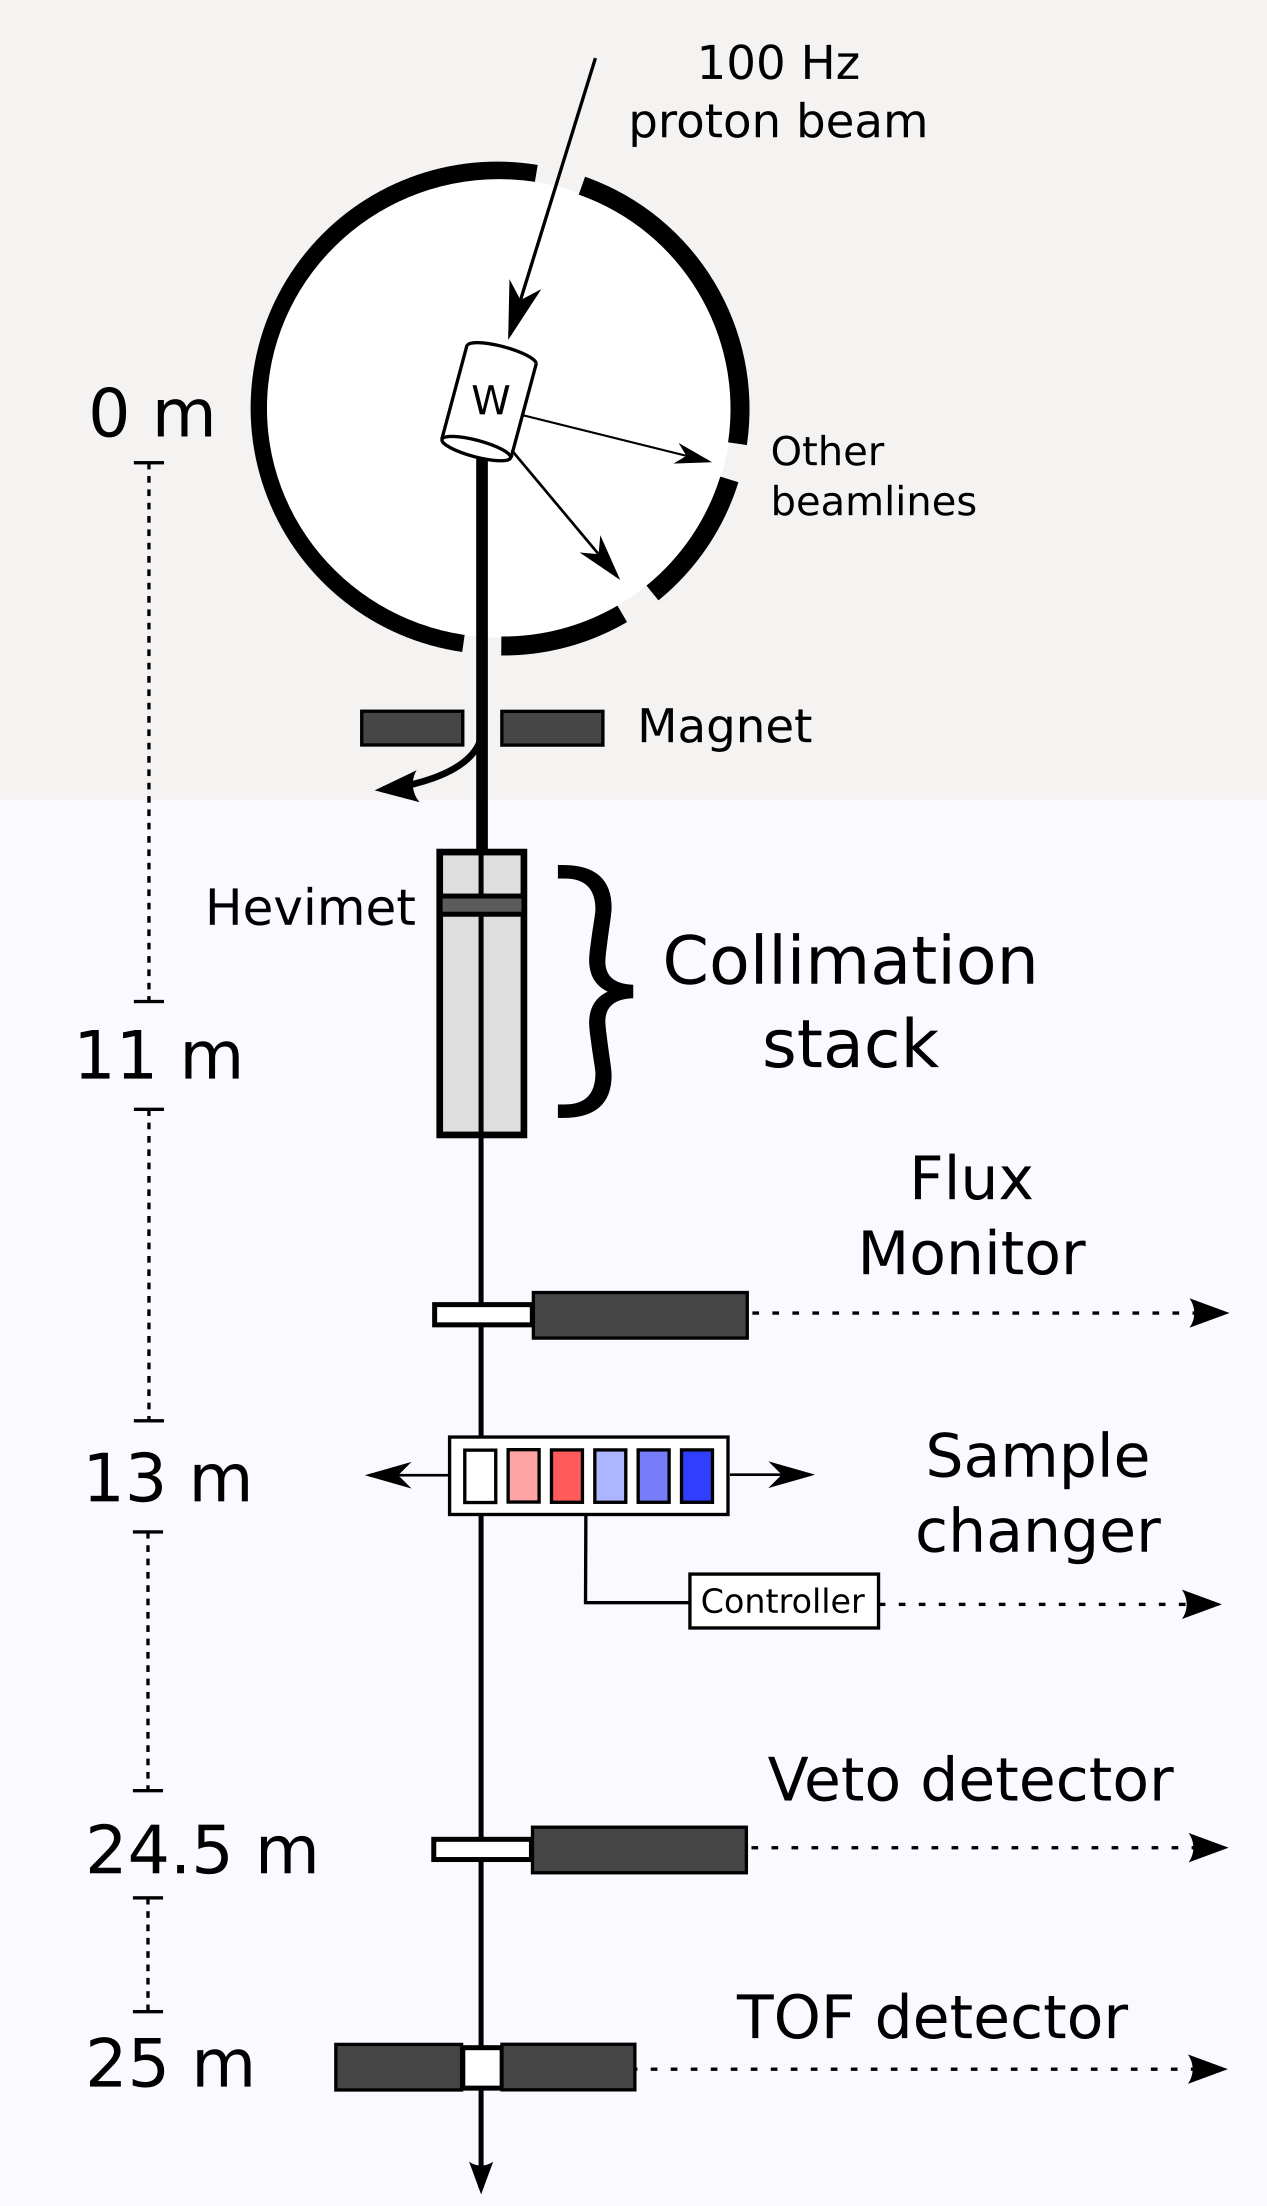
\includegraphics[width=0.4\textwidth]{figures/ExperimentalSetup.png}
    \caption[Layout of the 15R beamline at the WNR facility at LANSCE]
        {Layout of the 15R beamline at the WNR facility at LANSCE, with our
    experimental equipment indicated toward the bottom of the flight path.
    After a permanent magnet sweeps charged particles from the beam, neutrons and
    $\gamma$-rays are collimated to a 0.200'' beam en route to the
    detectors used in the experiment. Samples are cycled into and out of beam
    using a linear actuator with a period of 150 seconds. Times-of-flight (TOFs) are
    determined by the TOF detector and used to calculate neutron energy.
}
    \label{ExperimentalApparatus}
\end{figure}

\begin{figure}[h]
    \centering
    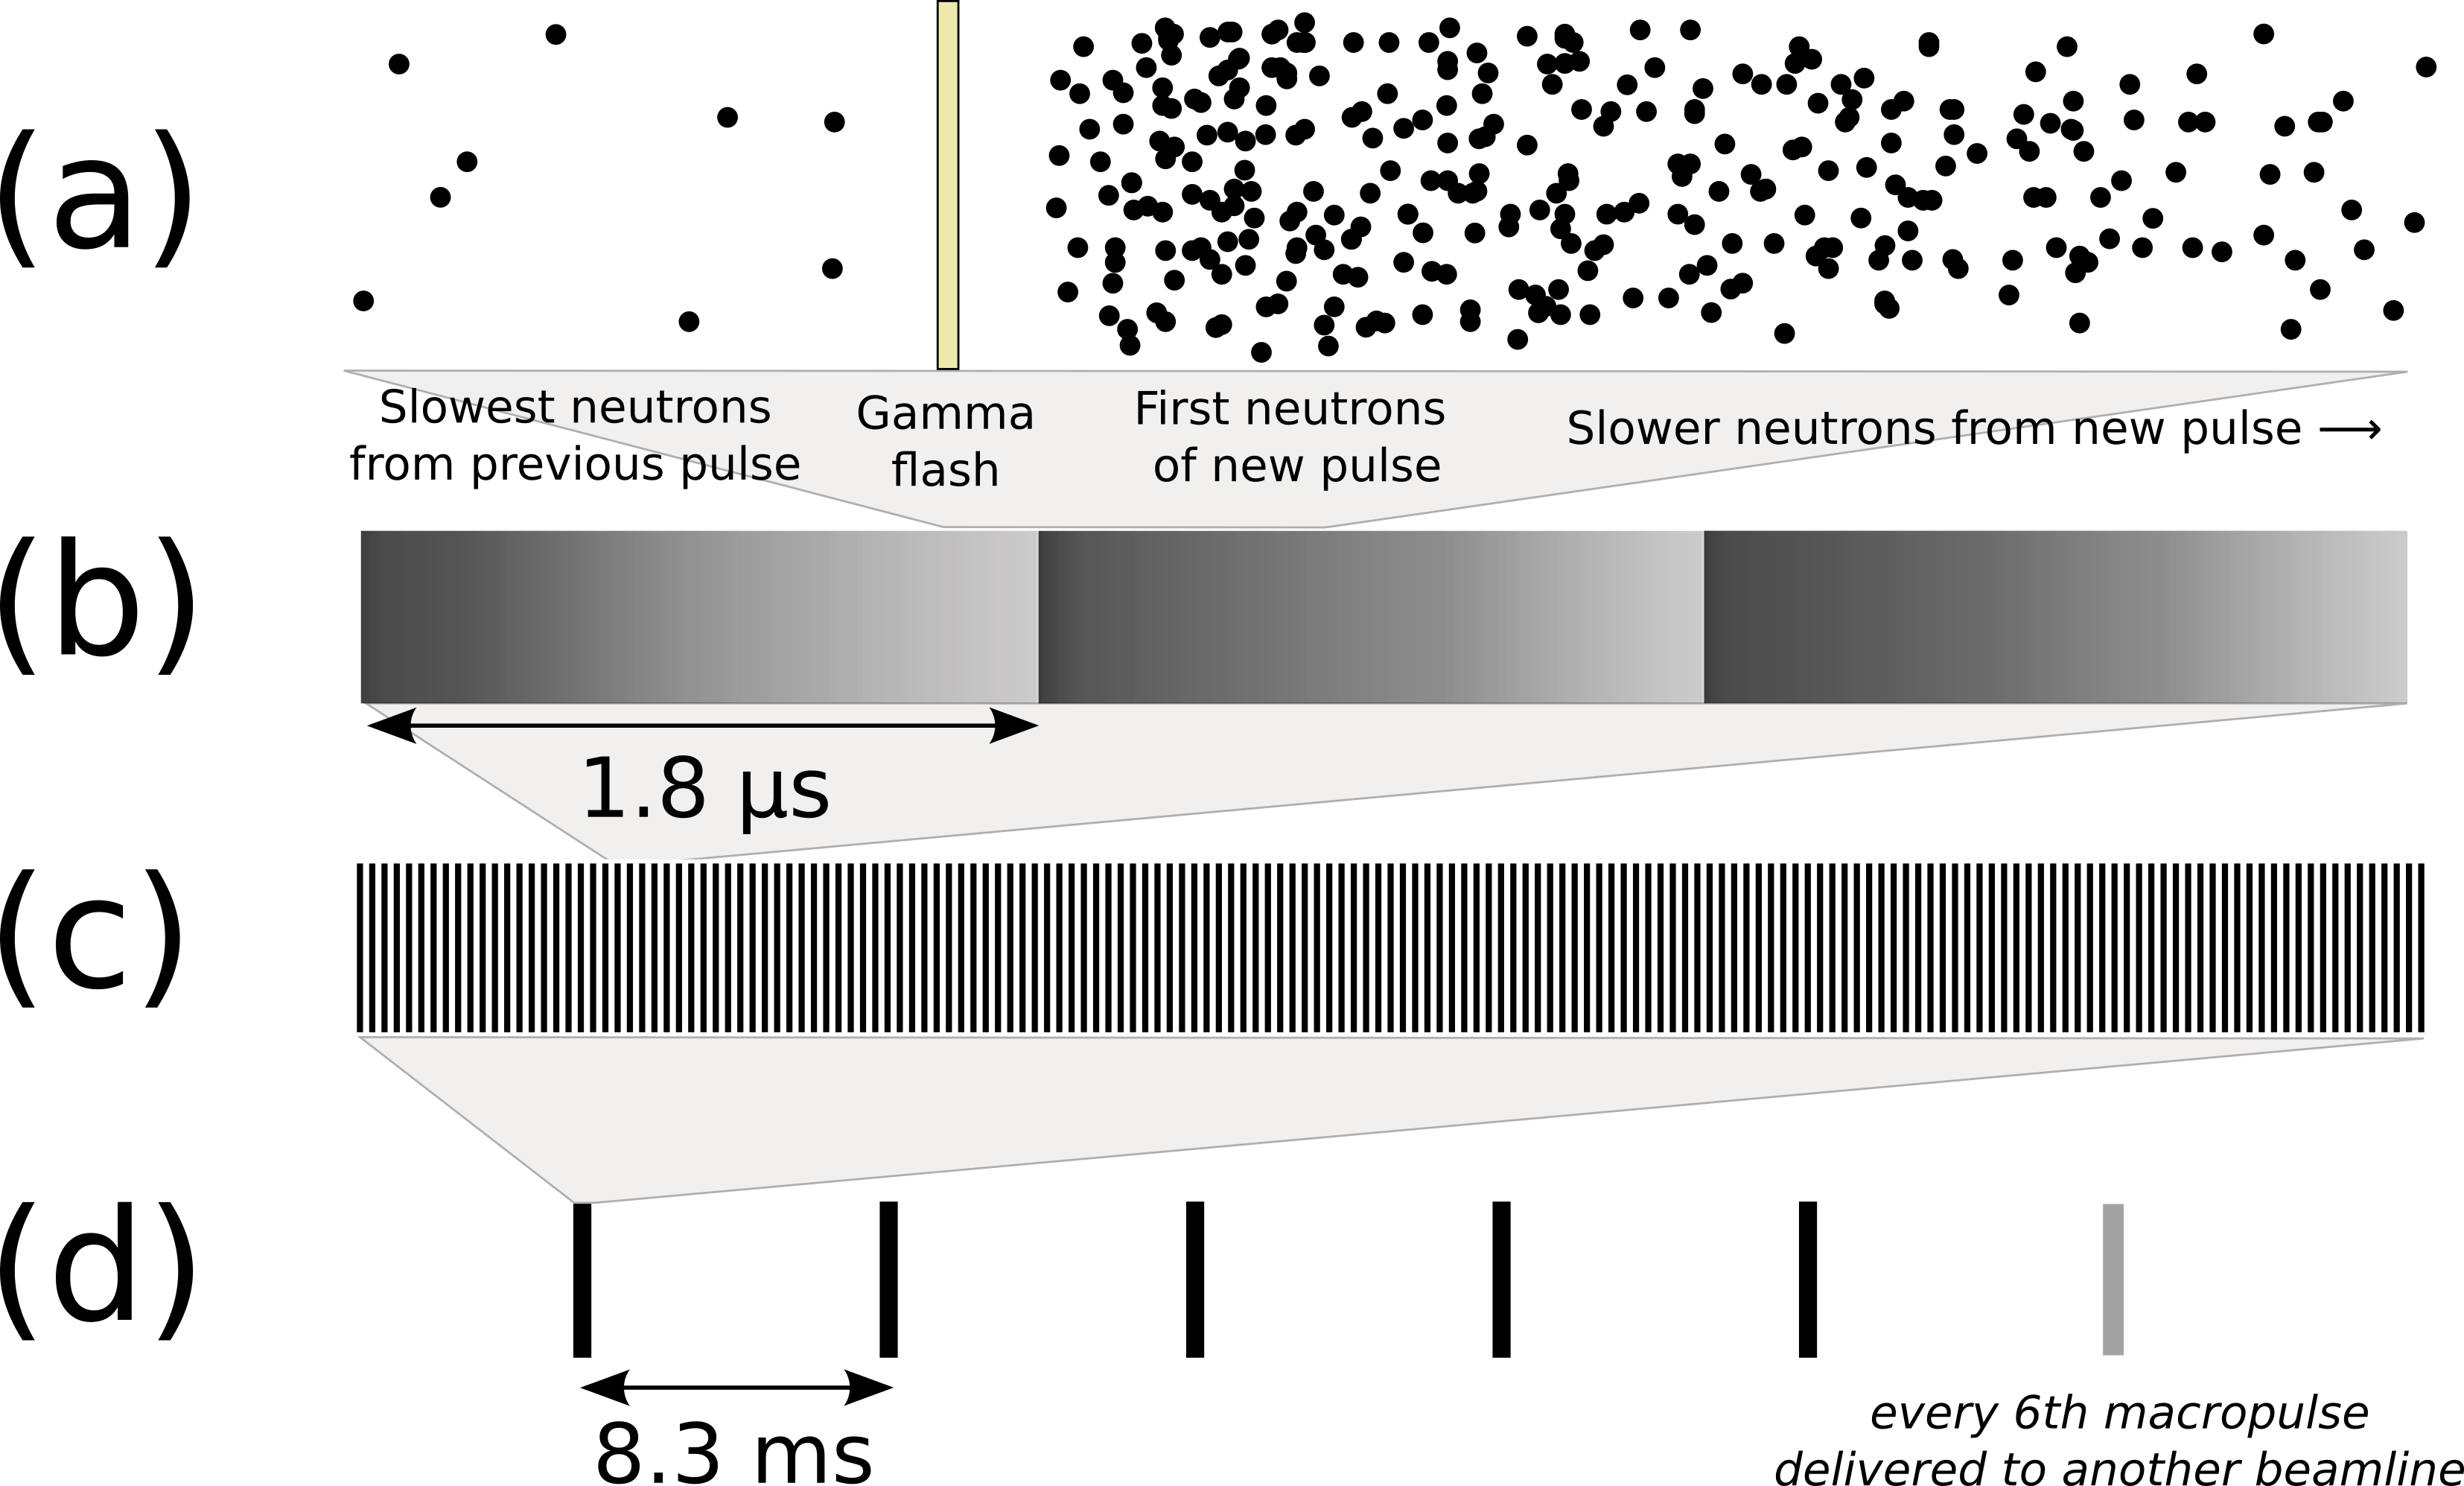
\includegraphics[width=0.8\textwidth]{figures/beamStructure.png}
    \caption[Pulsed structure of the neutron beam at the WNR facility]
    {
        Neutron beam structure at WNR facility.
        ``Macropulses" of protons (row d) are delivered to
        WNR's tungsten Target 4, where they generate neutrons by spallation.
        Each macropulse consists of
        $\approx$350 proton ``micropulses" (row c). Neutrons
        from each micropulse (row b) disperse in
        time as they travel along the flight path so that $\gamma$ rays and high-energy 
        neutrons catch up to low-energy ones from the previous pulse (row a).
    }
    \label{BeamStructure}
\end{figure}

\begin{figure}[h]
    \centering
    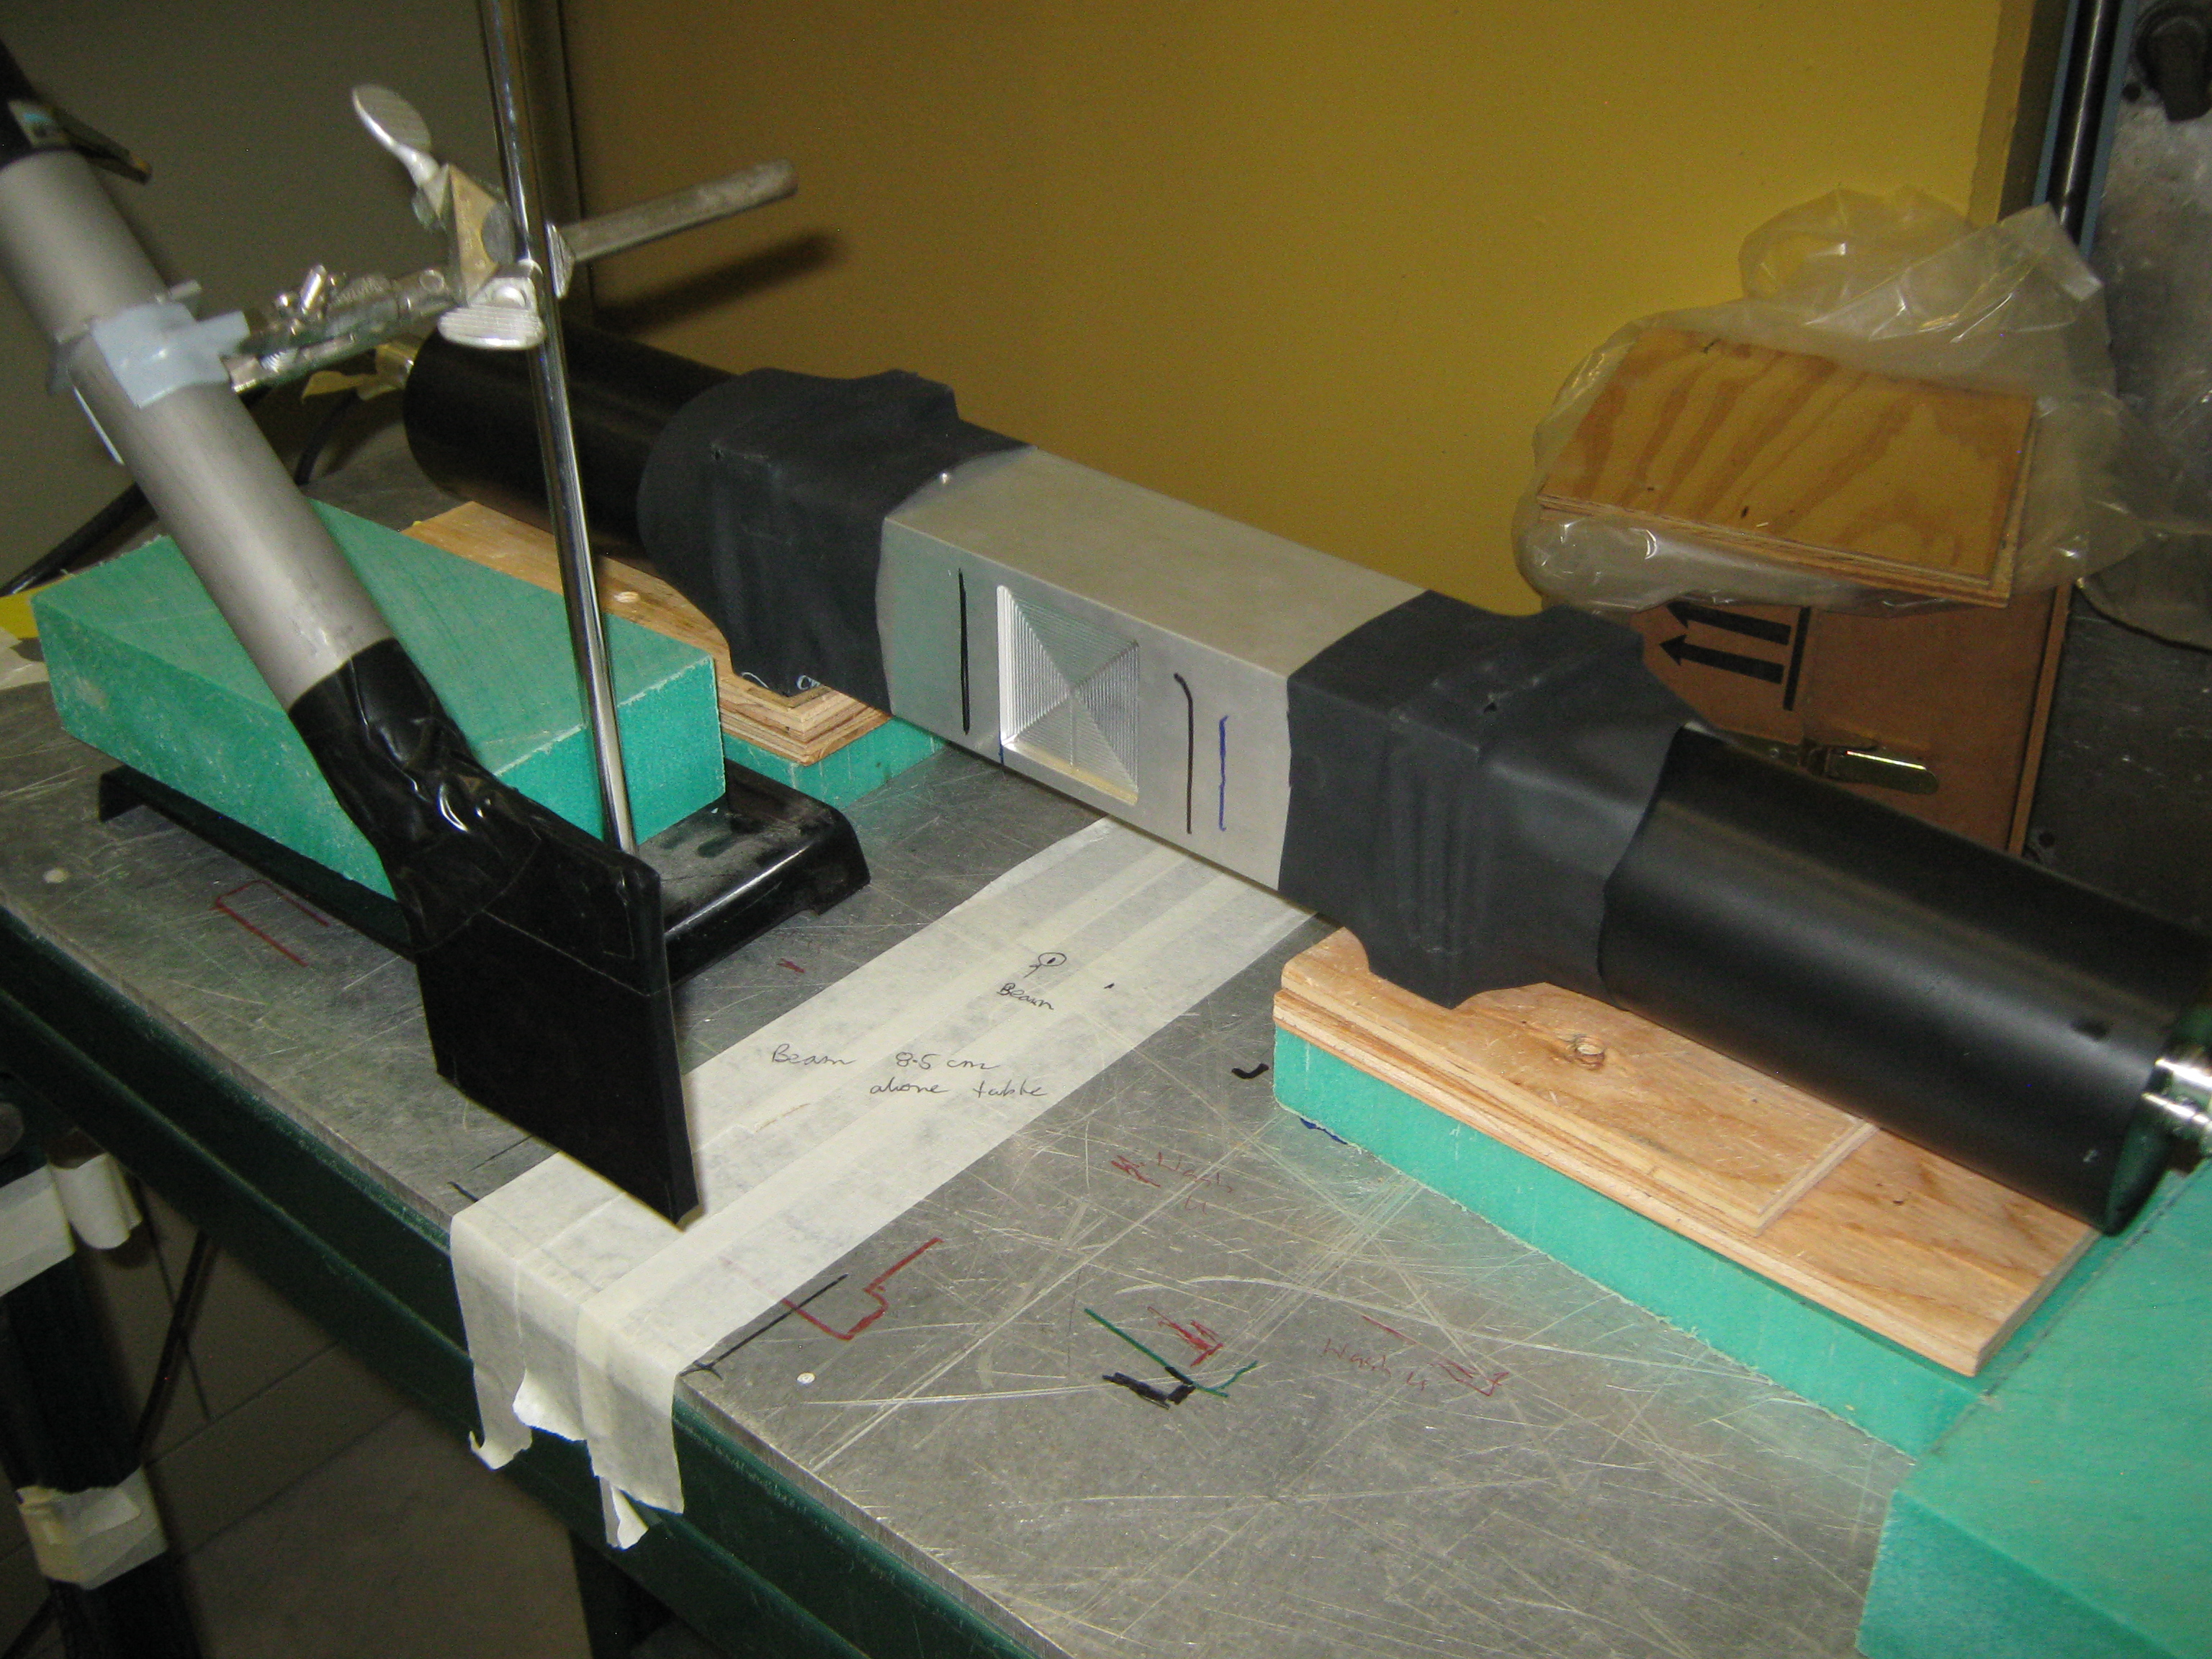
\includegraphics[width=0.45\textwidth]{figures/VetoAndTOFDetectors.jpg}
    \caption{Veto and time-of-flight detectors installed in the 15R beamline}
    \label{VetoAndTOFDetectors}
\end{figure}

\begin{figure}[h]
    \centering
    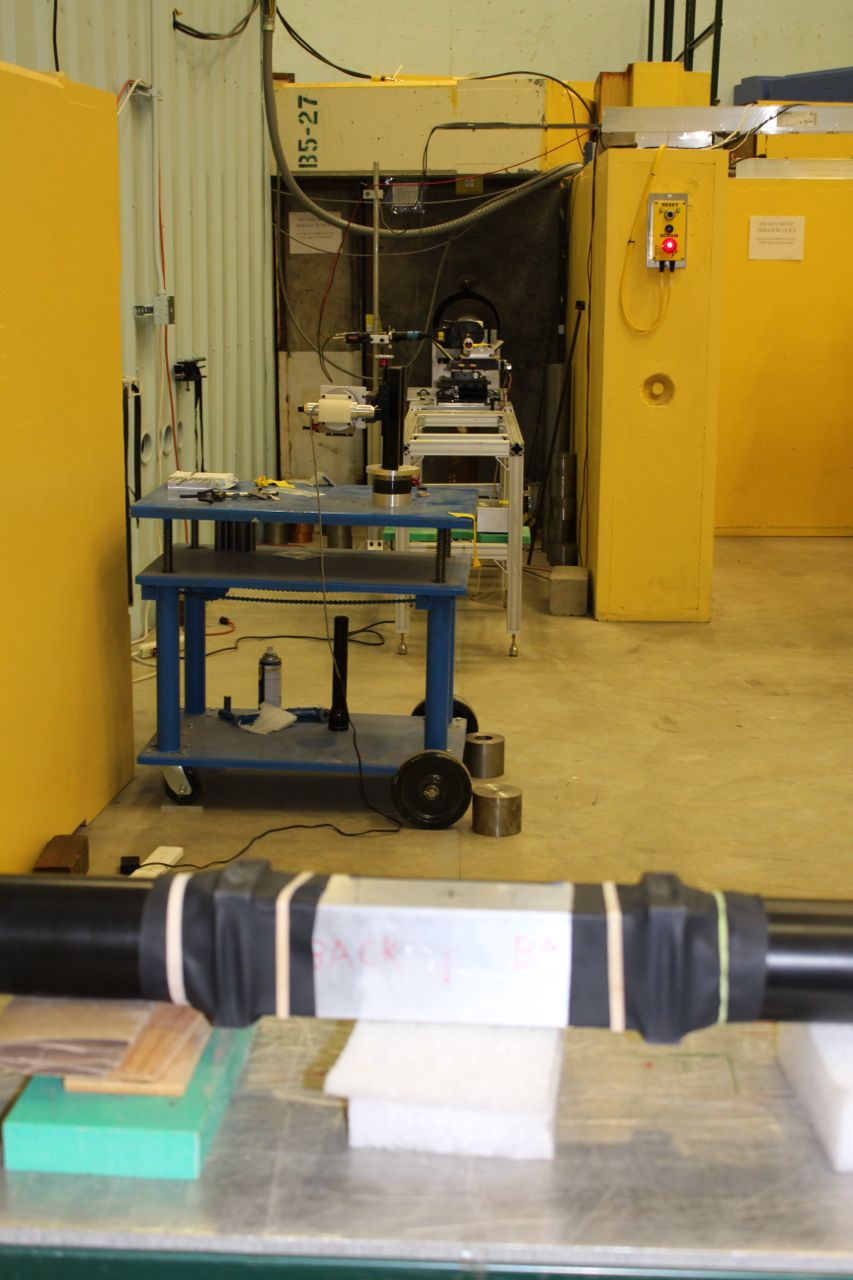
\includegraphics[width=0.45\textwidth]{figures/UpstreamFromTOFDetector.jpg}
    \caption{Overview of \tot\ experimental setup in the 15R beamline}
    \label{BeamlineUpstream}
\end{figure}

\begin{figure}[h]
    \centering
    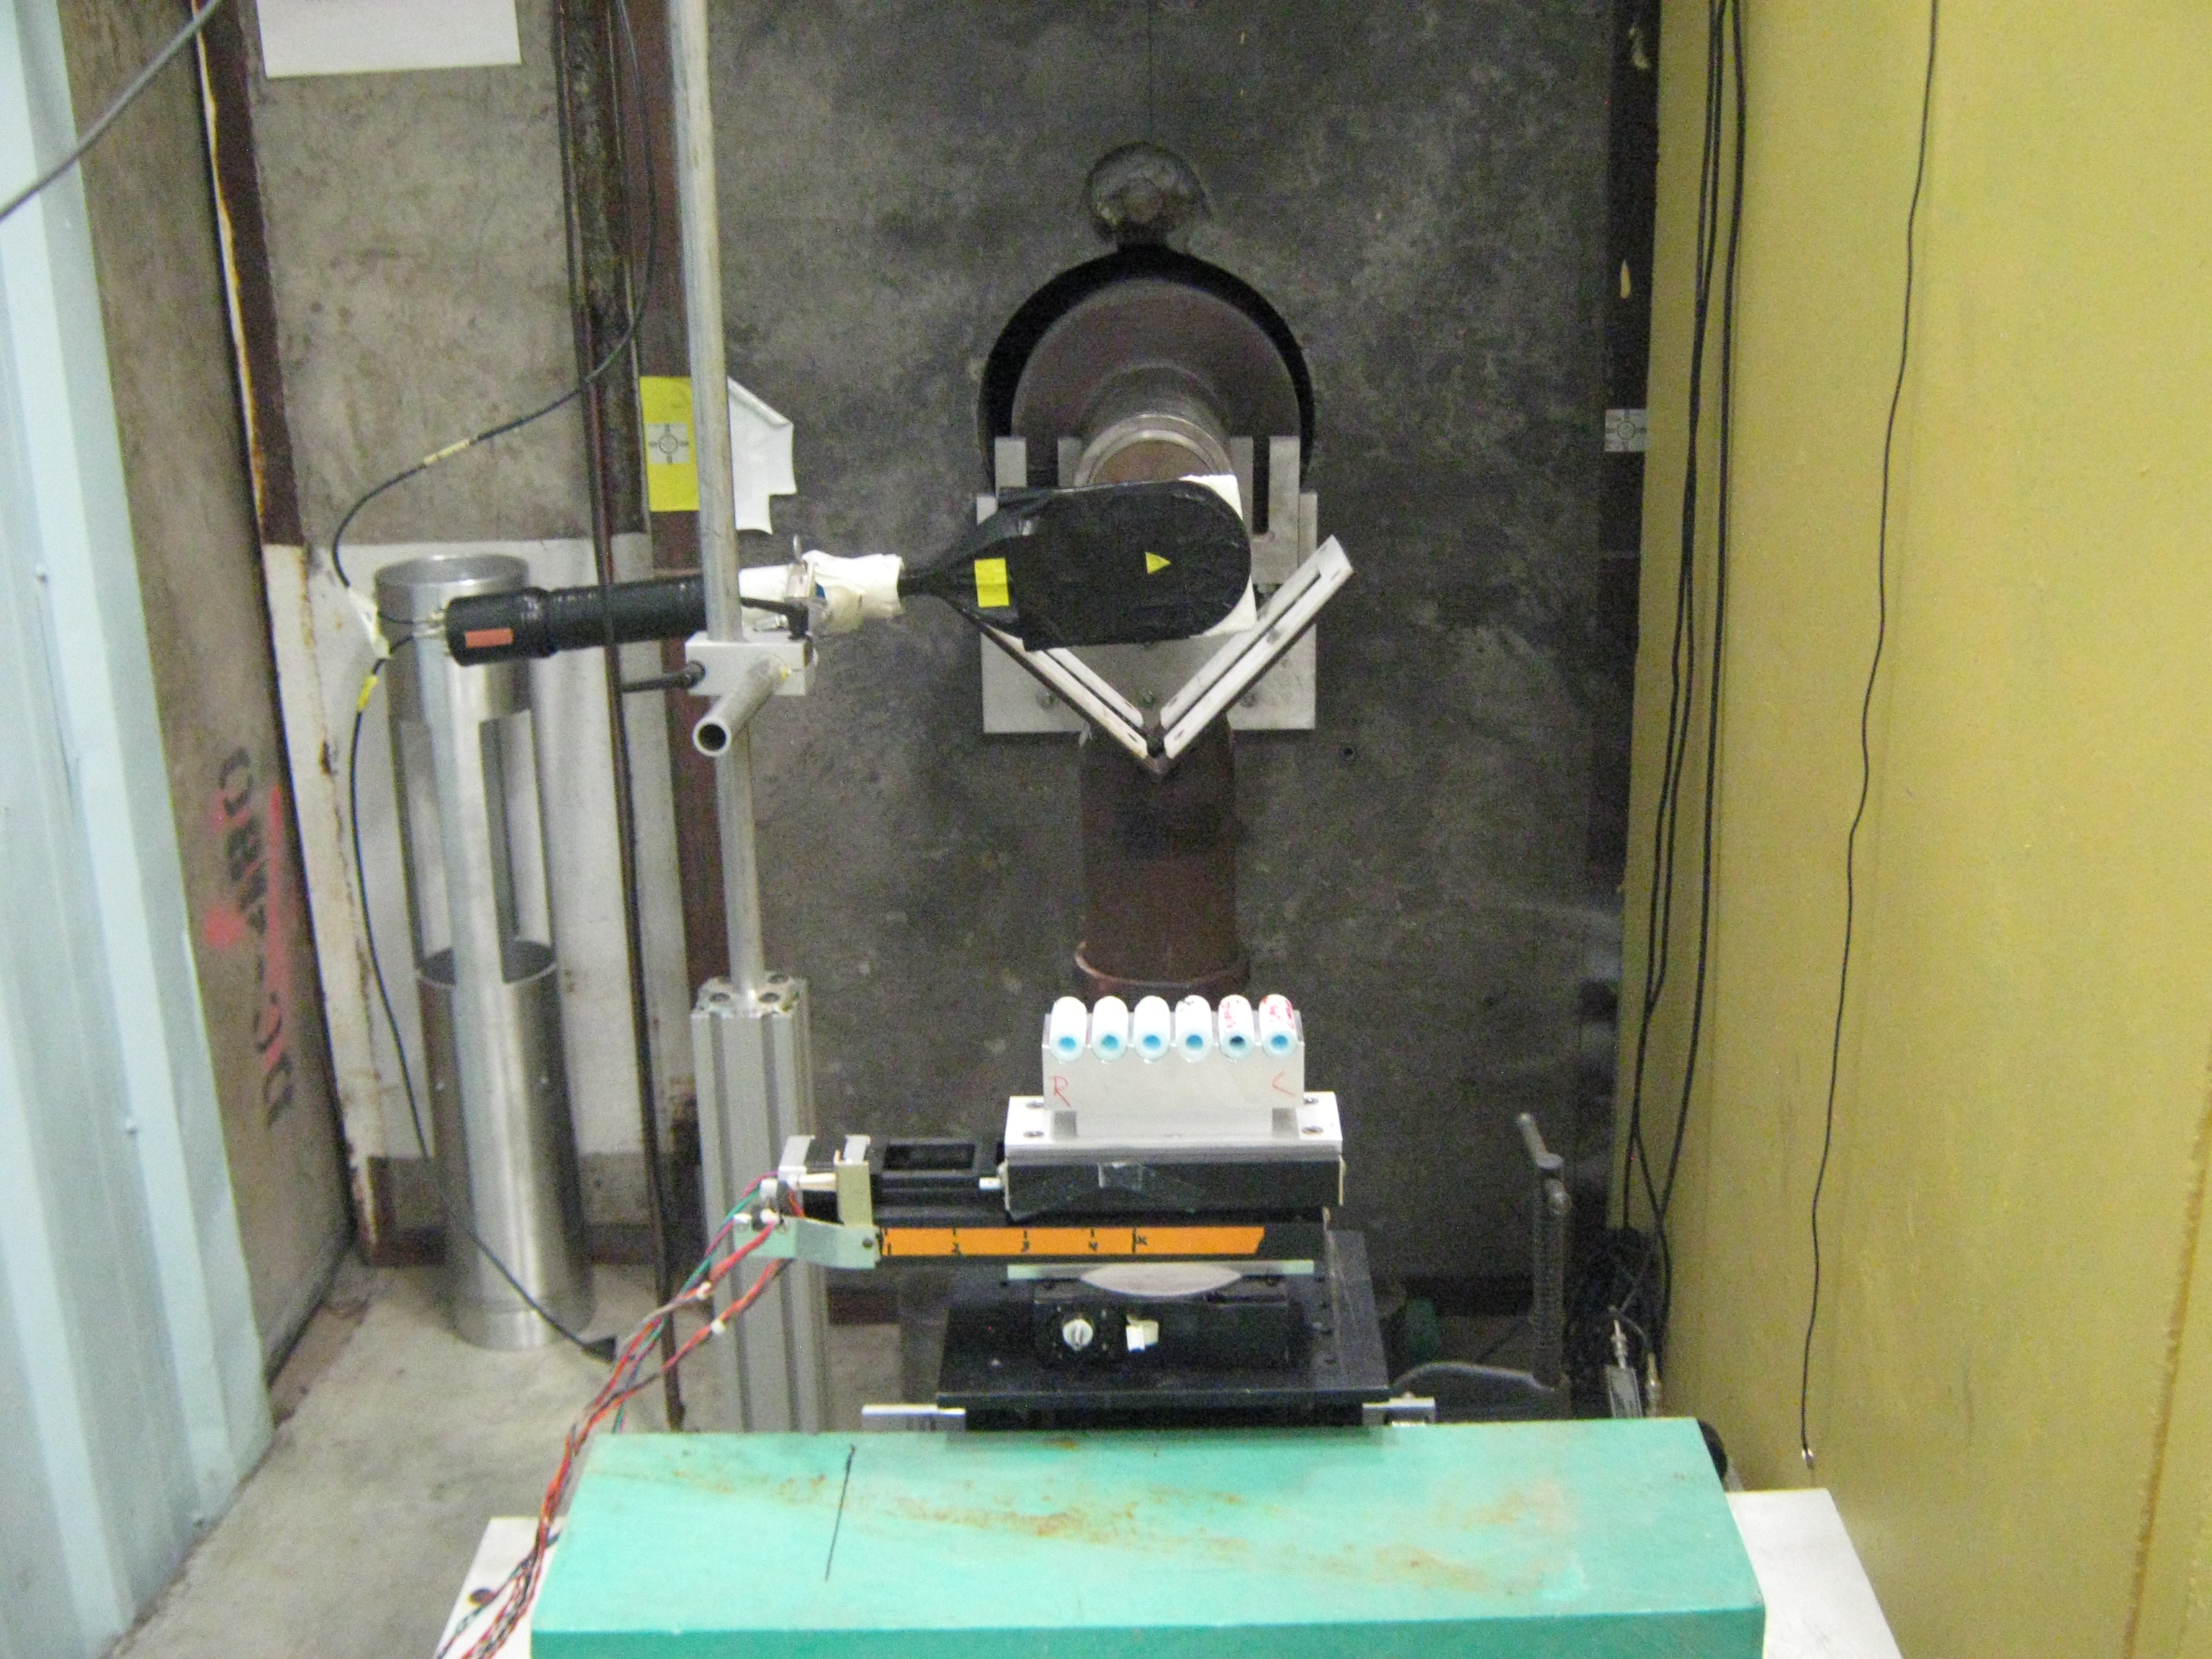
\includegraphics[width=0.45\textwidth]{figures/UpstreamTowardCollimator.jpg}
    \caption{Sample changer, monitor detector, and collimation stack}
    \label{BeamlineSampleChanger}
\end{figure}

The particular neutron beam structure at WNR dictates the energy range
achievable for \tot\ measurements (see Fig. \ref{BeamStructure}).
Proton pulse trains, called ``macropulses", are delivered to the tungsten target at 120 Hz.
Each macropulse consists of ~350 individual proton pulses, called ``micropulses", spaced 1.8 
$\upmu$s apart. Each micropulse consists of a single proton packet $<$1 ns wide when it 
arrives at the tungsten target that generates gamma rays and neutrons within a tight
temporal-spatial range. As neutrons from this micropulse travel along the beam path, 
high-energy neutrons separate in time from lower-energy neutrons so that neutron
energy can be determined by standard TOF techniques described in Chapter
\ref{TCSAnalysis} (see \cite{Moore1980} for additional details).
Because the $\gamma$ rays and high-energy neutrons from later micropulses can
overtake slower neutrons from an earlier micropulse, an important tradeoff
exists between measuring low and high-energy neutrons. The further the time-of-flight
detector is placed from the neutron source, the higher the minimum neutron energy that can be 
unambiguously resolved. However, placing the time-of-flight detector closer to the neutron source
increases the maximum instantaneous neutron flux at the start of each
micropulse, increasing the average per-event deadtime for the highest-energy
neutrons. A balance must be stuck between the detector thickness, the neutron
flux, the $\gamma$-ray flux, the time-of-flight detector distance, and the rate
of data acquisition.

A programmable sample changer with six positions
was used to cycle each sample into the beam at a regular interval of 150 seconds 
per sample. Once per macropulse, an analog signal from the sample changer was recorded to 
indicate its current position. The sample configuration for each run varied, but
generally all six positions on the sample changer were used. For the solid targets,
a typical configuration was to place an empty styrofoam sample sleeve in the
first sample-changer cradle as
the ``blank", the \cNat\ and \pbNat\ samples in the second and third
cradles, and the samples of interest (e.g., \niEight, \niNat, \niFour) in
the fourth, fifth, and sixth cradles. For water samples, an empty brass vessel
was placed in the first cradle to serve as the blank.

Due to beam divergence after collimation and the small diameter of the
samples, precise alignment of the sample changer was paramount. The sample
changer was placed on an adjustable table and roughly aligned by laser. For
precise alignment, a 2-inch aluminum cylinder with a
$\frac{1}{16}$-inch axial hole was placed
in the first position of the sample changer and a radiographic film placed
immediately posterior. The film was irradiated by the neutron beam for fifteen 
minutes and developed to show the alignment of the aluminum cylinder with the
beam profile. The position of the target changer was adjusted to improve alignment,
and the process was
iterated until alignment was satisfactory, ensuring that all neutrons
reaching the time-of-flight detector had to pass through the in-beam sample.
Figure \ref{SampleChangerAlignment} shows a radiogram confirming alignment of all
sample changer positions within 1 mm.

The beam flux of each macropulse, required to normalize absolute cross sections, was continuously
monitored by the flux monitor detector. The veto detector immediately upstream
of the time-of-flight detector was used to reject time-of-flight events from
charged-particle production in the samples and in air along the flight path. The
left and right PMTs of the time-of-flight detector were gain-matched and a
0.5-ns cable delay was introduced on the right PMT signal to improve the
time-matching between the left and right signals.

\section{Data Acquisition}
Signals from all detectors and the sample changer were relayed to an 8-channel, 500-MHz CAEN 
DT-5730
waveform digitizer as shown in Fig. \ref{TCSLogicDiagram}. Custom software was used to run the 
digitizer in two complementary modes, referred to as ``DPP mode" and ``Waveform 
mode". In DPP mode, triggers were initiated by the digitizer's onboard
peak-sensing firmware. For each trigger, several quantities were recorded: the trigger 
timestamp, two charge integrals over the detected peak with different
integration ranges (32 ns for the short integral, 100 ns for the long integral),
and a 96-ns portion of the raw digitized waveform, referred to as a ``wavelet".
The timestamp was stored as two components: a 48-bit timestamp with 2 ns
resolution, and 10-bit "fine time" within the 2 ns coarse time bin period.
DPP mode was used for the vast majority of the 
experiment and accounts for $\approx$99\% of the total data volume. In waveform mode, 
the digitizer performs no peak-sensing and was externally triggered. Upon 
triggering, the trigger timestamp and a very long wavelet (60 $\upmu$s) 
were recorded. While waveform mode data accounts for only $\approx$1\% of the total data, 
the instantaneous data rate is much higher than in DPP 
mode because hundreds of $\upmu$s of consecutive waveform samples are 
stored. Roughly once every three seconds, the digitizer was switched to 
waveform mode for one macropulse, then switched back to DPP mode as quickly as
possible (within 10-40 ms, depending on run configuration). When the buffer for
any channel filled, all buffers were read out by optical link to a flash memory
drive of the data acquisition computer, minimizing the downtime of the digitizer
due to data readout.

Because we had fast digital-signal-processing technology available, we were able
to perform event detection and processing in a fundamentally-different way
compared to analog-mediated approaches. This is worth mentioning
here as it enabled a dramatic reduction, over an order of magnitude, in the size of the
samples required compared to previous measurements at the same facility. The reasons
for our approach and tradeoffs are
described in Section \ref{DeadtimeCorrection} of Chapter \ref{TCSAnalysis}.

\begin{figure}[h]
    \centering
    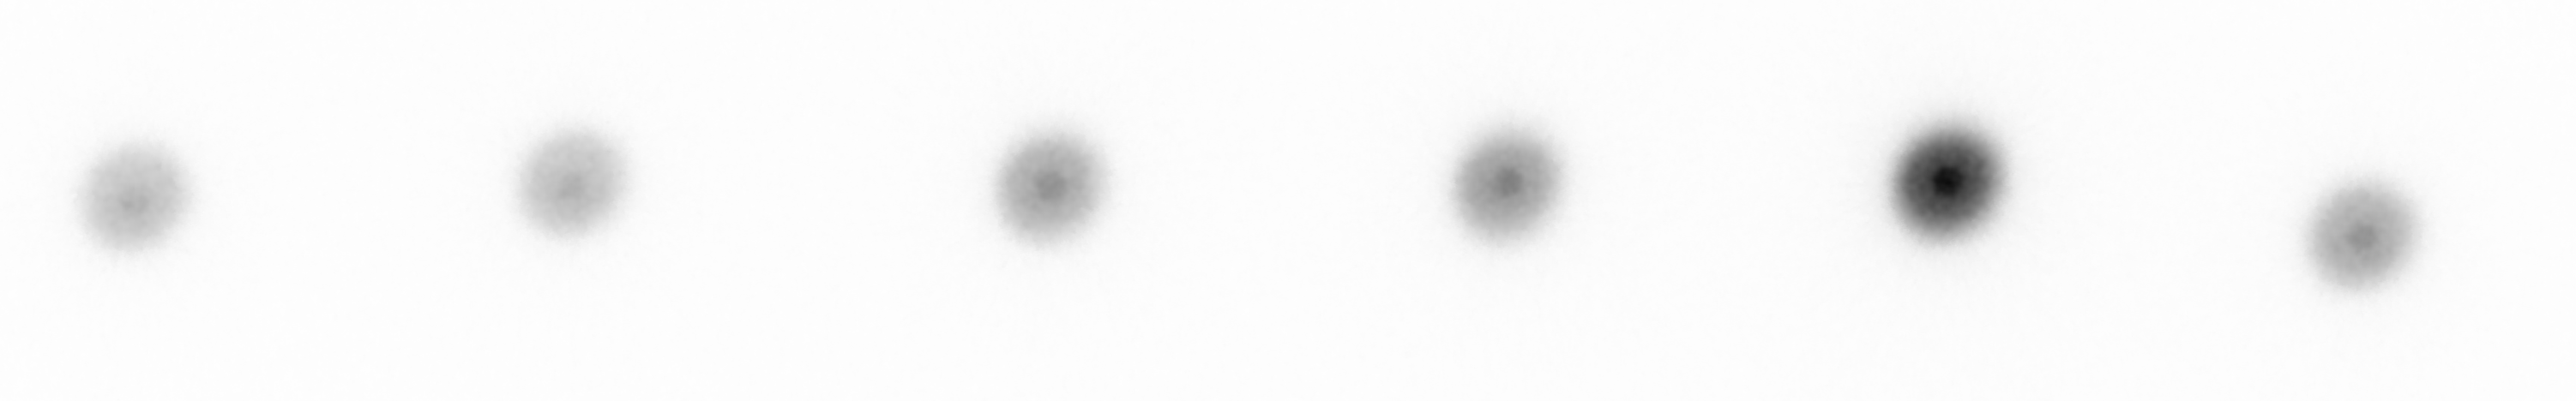
\includegraphics[width=0.8\textwidth]{figures/TargetChangerAlignment.png}
    \caption{Precision sample alignment via radiographic film}
    \label{SampleChangerAlignment}
\end{figure}

\begin{sidewaysfigure}[h]
    \centering
    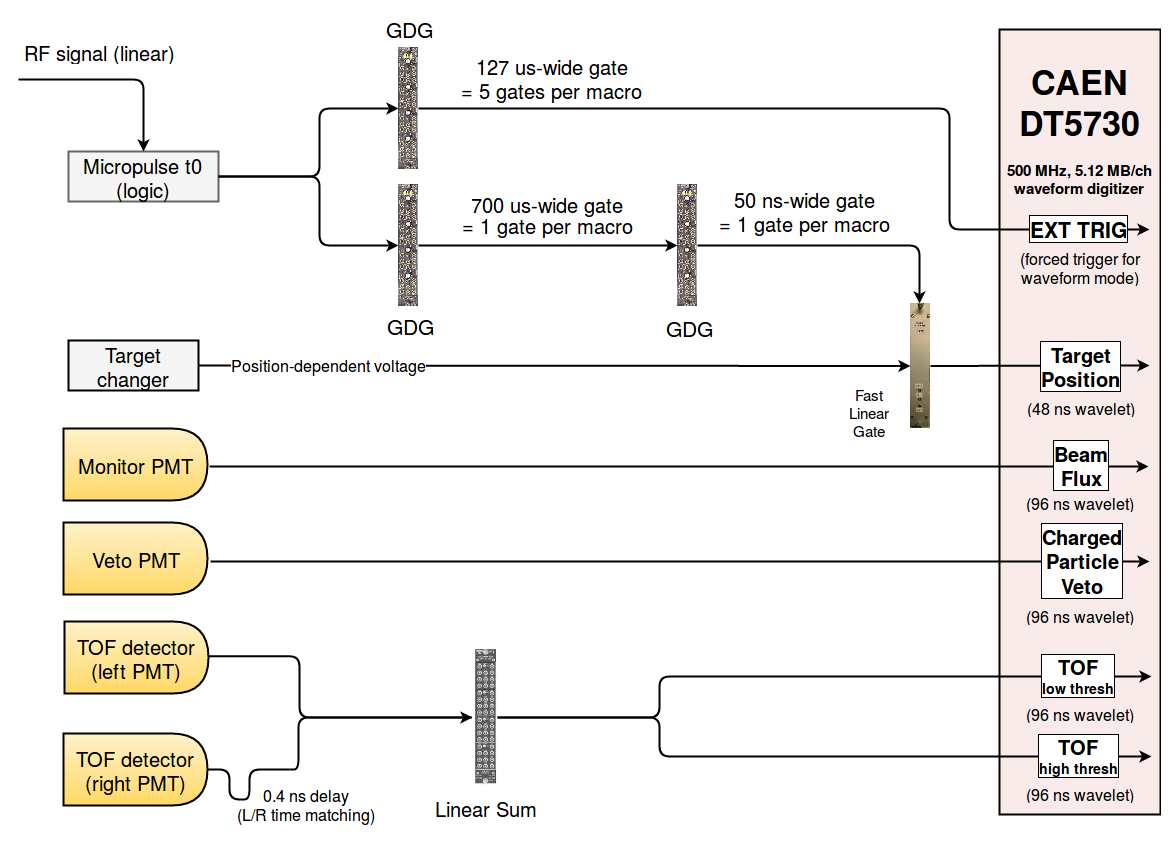
\includegraphics[width=0.9\textwidth]{figures/TCSLogicDiagram.png}
    \caption[Logic diagram for neutron \tot\ data acquisition]
    {Details on logic diagram}
    \label{TCSLogicDiagram}
\end{sidewaysfigure}

\afterpage{\clearpage}
